\documentclass{article}


\usepackage{graphicx}
\usepackage{url}
\usepackage{hyperref}
\usepackage{amsmath}
\usepackage{amssymb}
\usepackage{tipa}
\usepackage{mathtools}
\usepackage{caption}
\graphicspath{{./}}



\hypersetup{
	colorlinks=true,
	urlcolor=blue
}

\usepackage[margin=0.7in]{geometry}
\linespread{1.25}

\title{\fontfamily{bch}\selectfont\Huge Graph Theory Homework v1}
\author{\Large Petrov Maksim M3100}
\date{\Large \today}


\begin{document}
	\fontsize{14pt}{16pt}\selectfont
	\maketitle
	
	\section*{Tools and source files}
	Some problems were solved using \href{https://www.minizinc.org/software.html}{MiniZinc Software}. \href{https://www.minizinc.org/doc-2.7.0/en/index.html}{The MiniZinc Handbook} contains detailed instructions on how to run .mnz models and use .dzn data files. In this homework, some models use an adjacency matrix (g.dzn), other models use a list of edges (edges.dzn), others use a list of edges and the number of vertices (edges and v num.dzn). \\\\
	Some of the calculations were done (and the source code for graphviz was obtained) using console C++ applications built with a help of CMake. As the .exe file is located at {\textless}src folder{\textgreater}/Build/Debug, all input and output .txt files in the code begin with '../../' as it's convenient to work with them in the src folder just in IDE.\\\\
	To visualise the graphs, \url{https://dreampuf.github.io/GraphvizOnline/} was used (all graphs visualized using fdp engine).\\\\
	All source files can be found in \href{https://github.com/fish-from-SanDiego/GraphTheoryHW}{HW github repository}:
	MiniZinc files in 'mnz' folder, 'eu.txt' file for the list of the countries, 'tree', 'G', 'dist' and 'G\textbf{\_}star' for C++, 'tex' for \TeX and, finally, 'graphs' for the graphviz templates of $\mathcal{G}^*$, $\mathcal{G}$ and the tree.
	\newpage
	\section*{Task 1}
	The file 'eu.txt' contains a list of European countries, sorted lexicographically, and their \href{https://en.wikipedia.org/wiki/ISO_3166-1_alpha-2#:~:text=ISO%203166%2D1%20alpha%2D2%20codes%20are%20two%2Dletter,special%20areas%20of%20geographical%20interest.}{alpha-2 codes}. The vertices (countries) were labeled in order in this list and by adding alpha-2 code. $\mathcal{G} = \mathcal{G}^*[V(\mathcal{G}^*)\setminus \{\textmd{GB, IS, IE, CY, MT\}}]$. It's also assumed that Spain does not border the UK via Gibraltar.\\\\
	(a) As the only way to minimize number of intersections in the graphviz fdp graph is manually changing the order of nodes in the code and setting 'pos' attribute (which not always works properly) there is still a small number of redundant intersections.
	\begin{figure}[h]
		\centering
		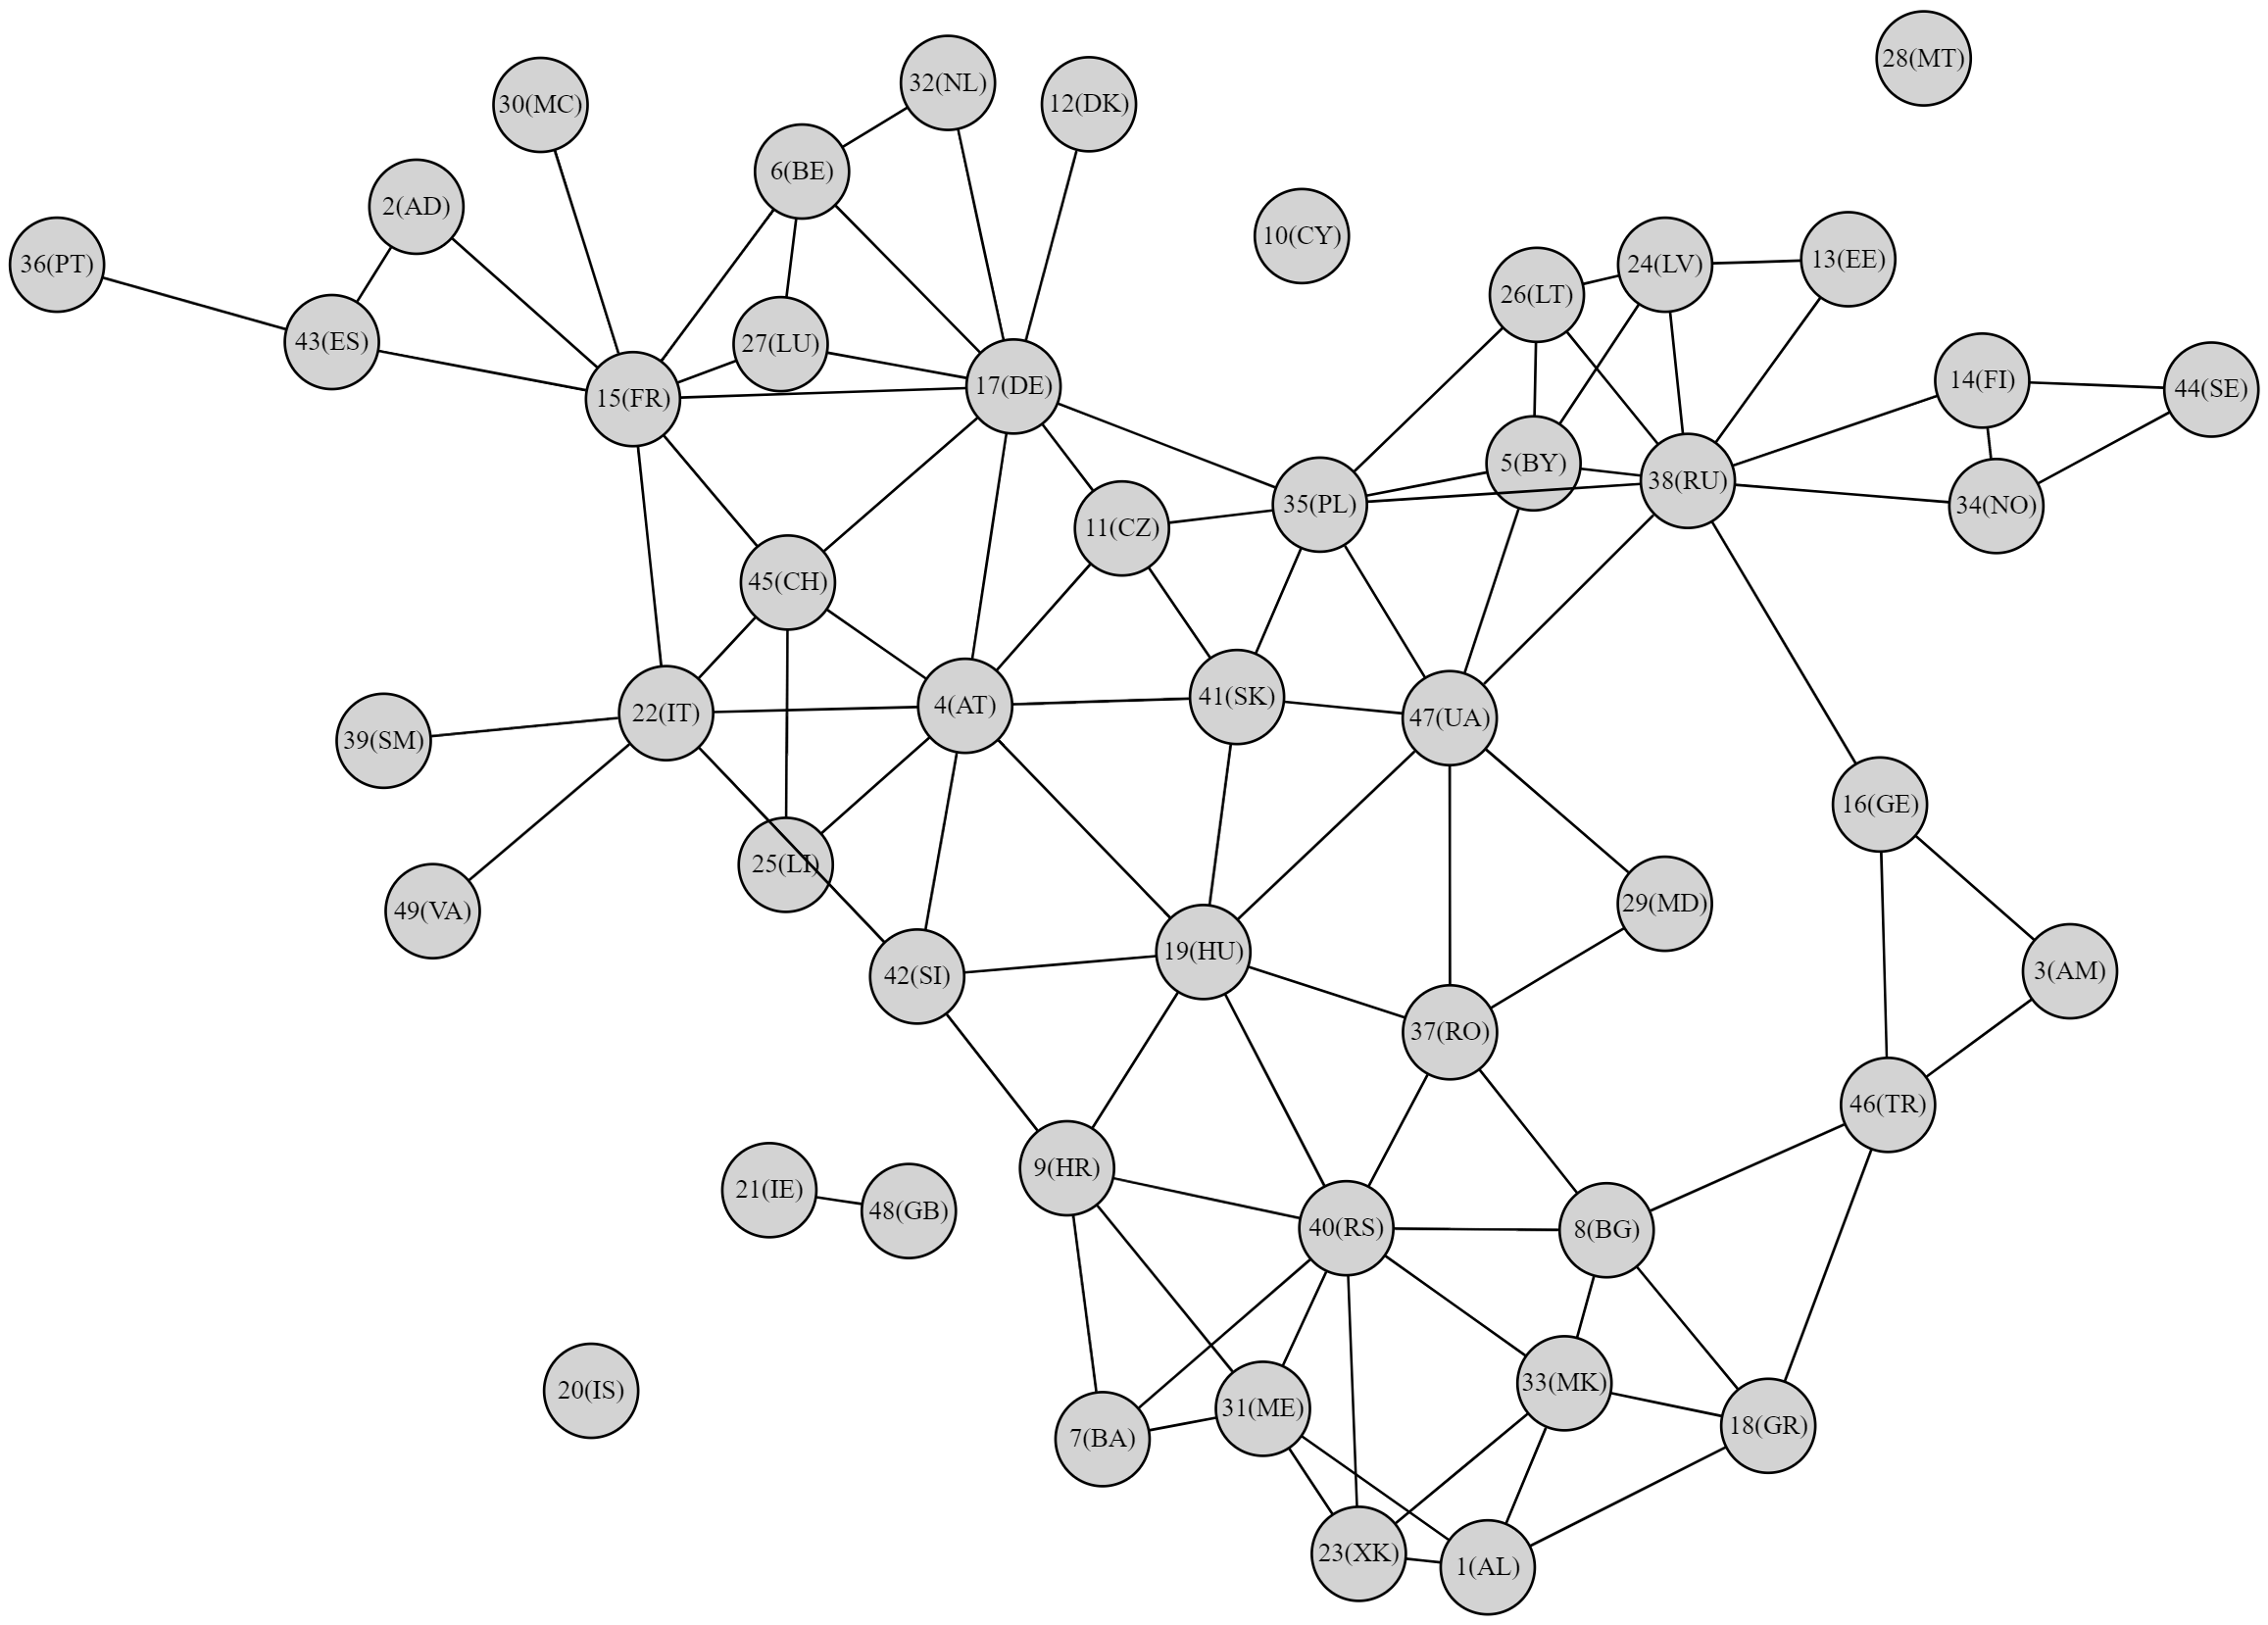
\includegraphics[width=1\textwidth]{G_star.png}
		\caption{$\mathcal{G}^*$ visualization}
	\end{figure}\newpage
	\begin{figure}[h]
		\centering
		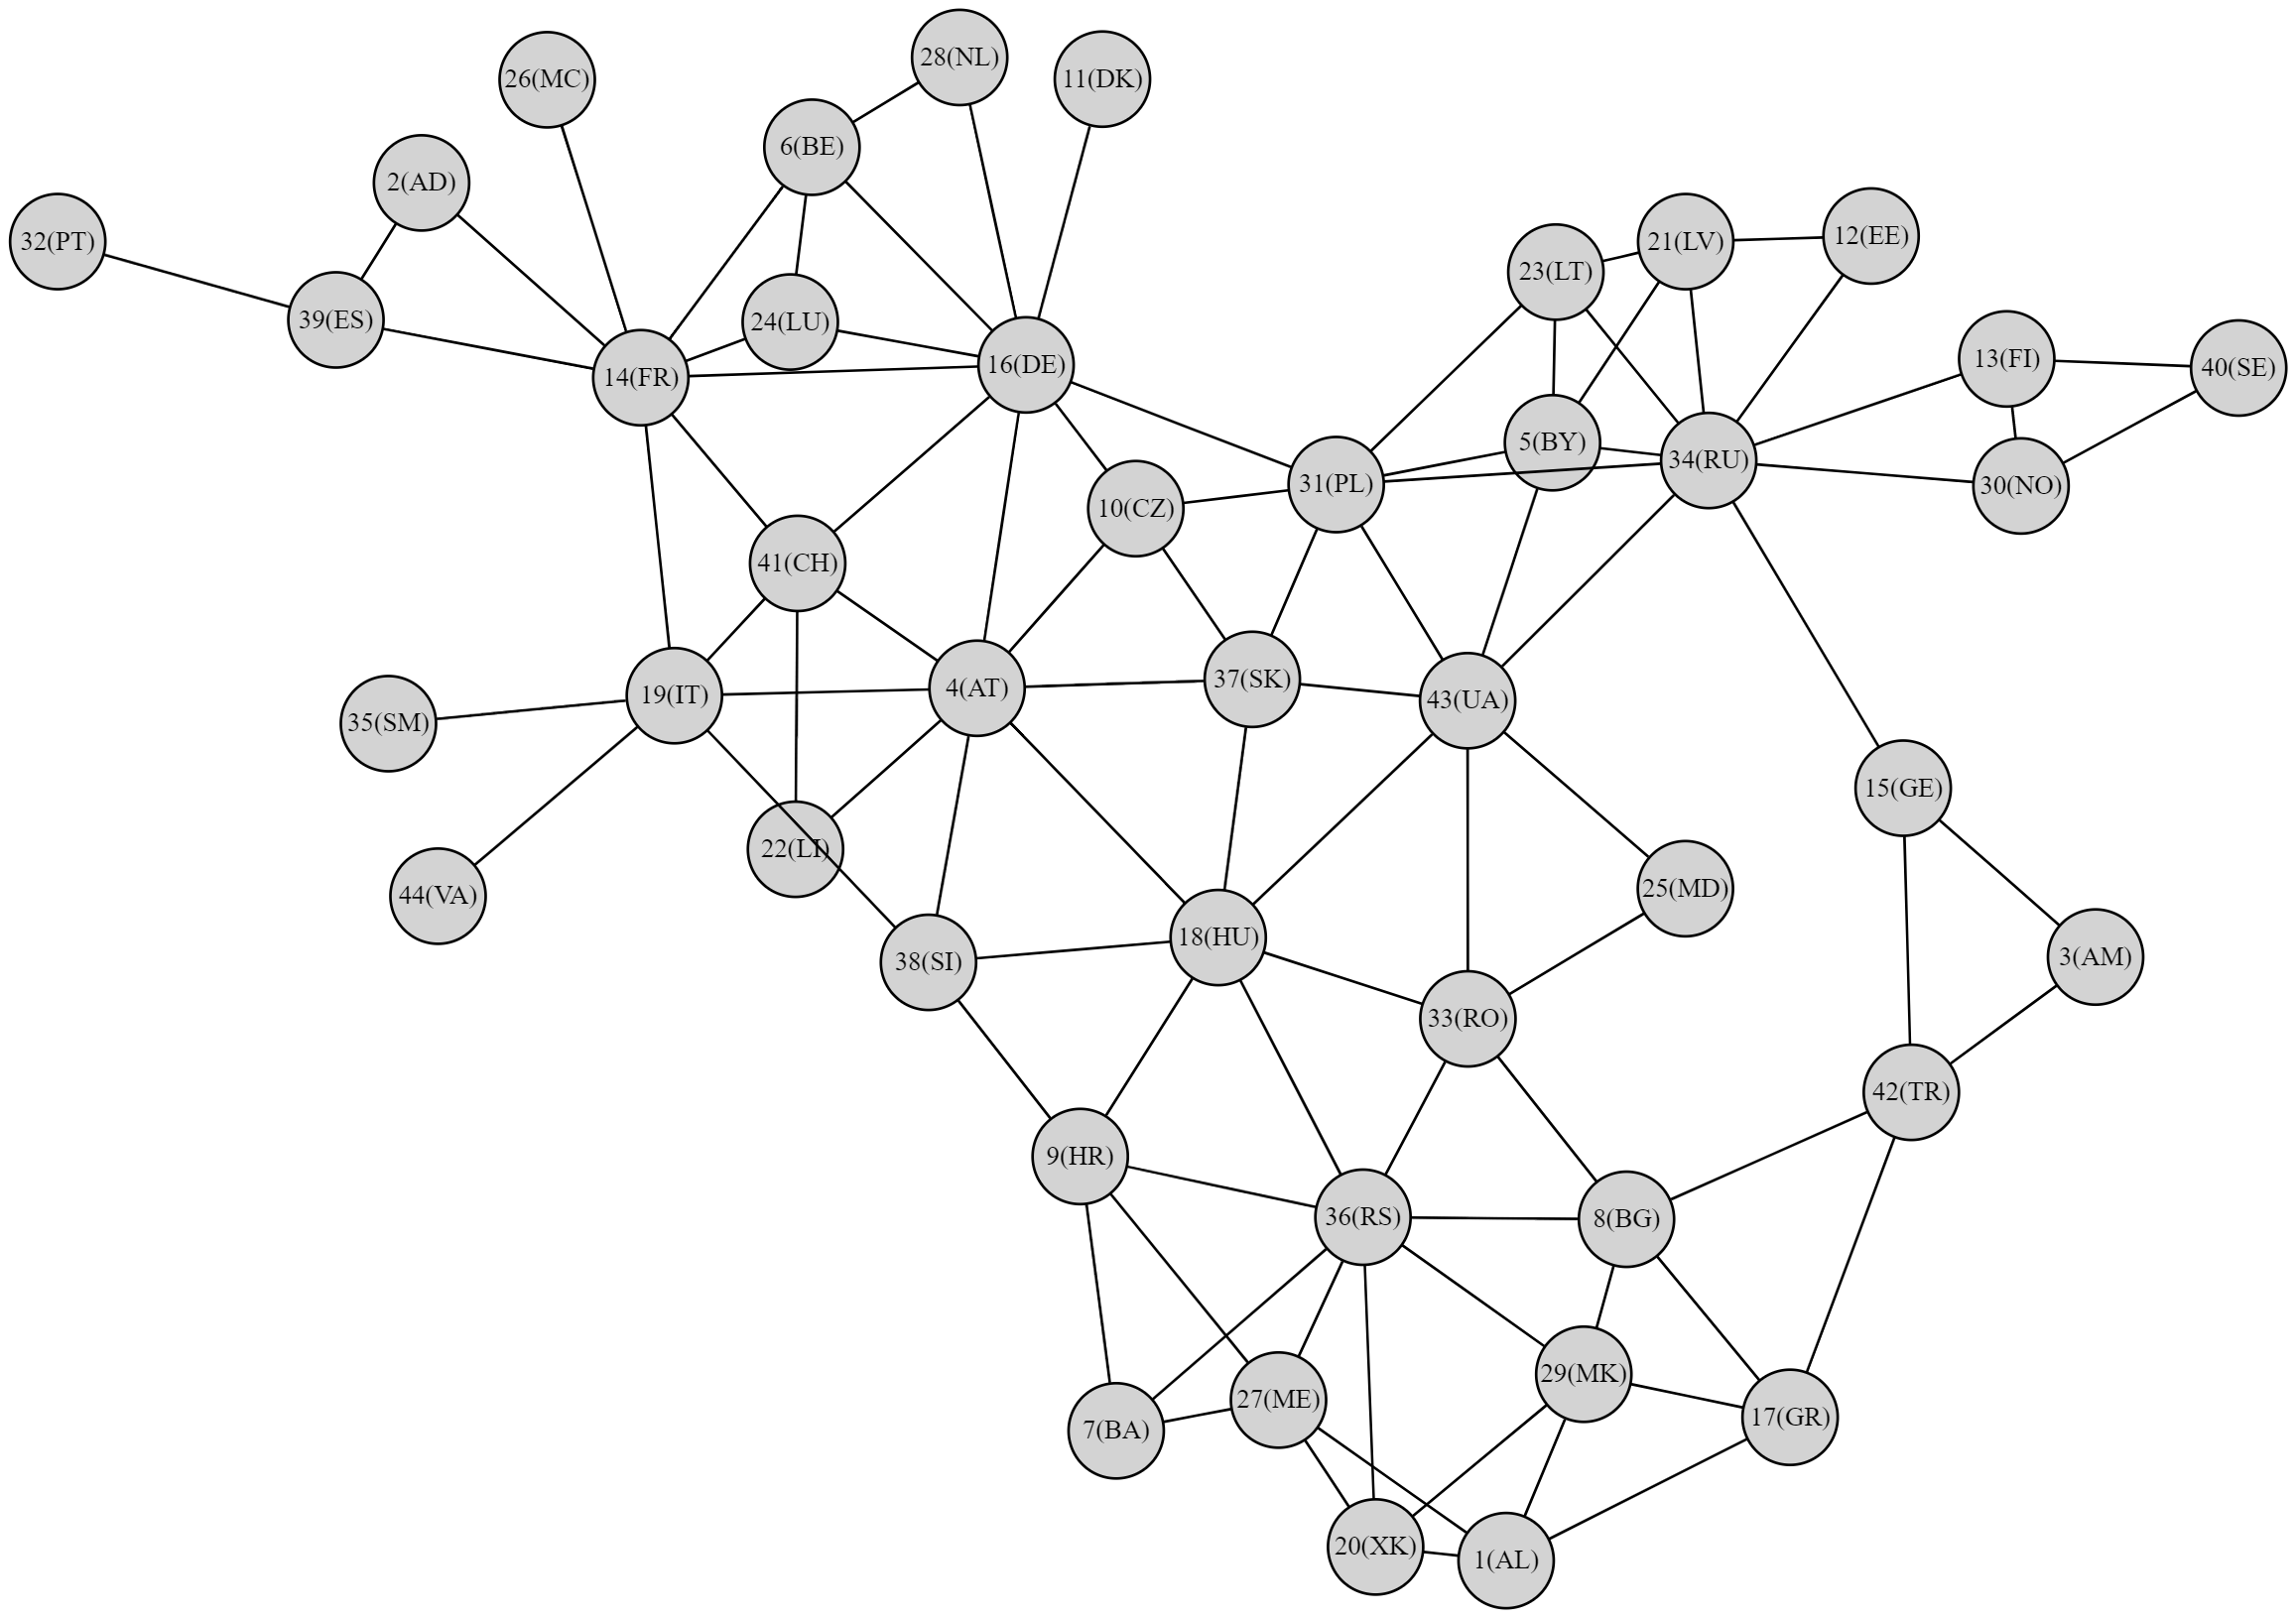
\includegraphics[width=1\textwidth]{G.png}
		\caption{$\mathcal{G}$ visualization}
	\end{figure}\newpage
	(b) Hereinafter vertices of $\mathcal{G}$ have labels different from labels in $\mathcal{G}^*$, so technically it's not subgraph as the labeling function has changed, but it's much more convenient to work with the graph in which vertices are labeled with $1..|V|$ and it's not so difficult to recover original labels as their second parts(alpha-2 codes) haven't changed.
	\\$|V| = 49,~ |E| = 91,~ \delta(\mathcal{G}) = 1$ ($\delta(\mathcal{G}) > 0$ as the graph is connected, e.g. degree of 32(PT) = 1), $\Delta(\mathcal{G}) = 9$ (for 34(RU)), $\textmd{rad}(\mathcal{G}) = 5,~\textmd{diam}(\mathcal{G}) = 8,~\textmd{girth}(\mathcal{G}) = 3,~|\textmd{center}(\mathcal{G})| = 13,~\varkappa(\mathcal{G}) = 1,~\lambda(\mathcal{G}) = 1$. The example of cycle with 3 edges is\\ RS-RO-BG; rad, diam and center are calculated using program from 'dist' folder, it's enough to delete ES or ES-PT to make graph disconnected.
	\begin{figure}[h]
		\centering
		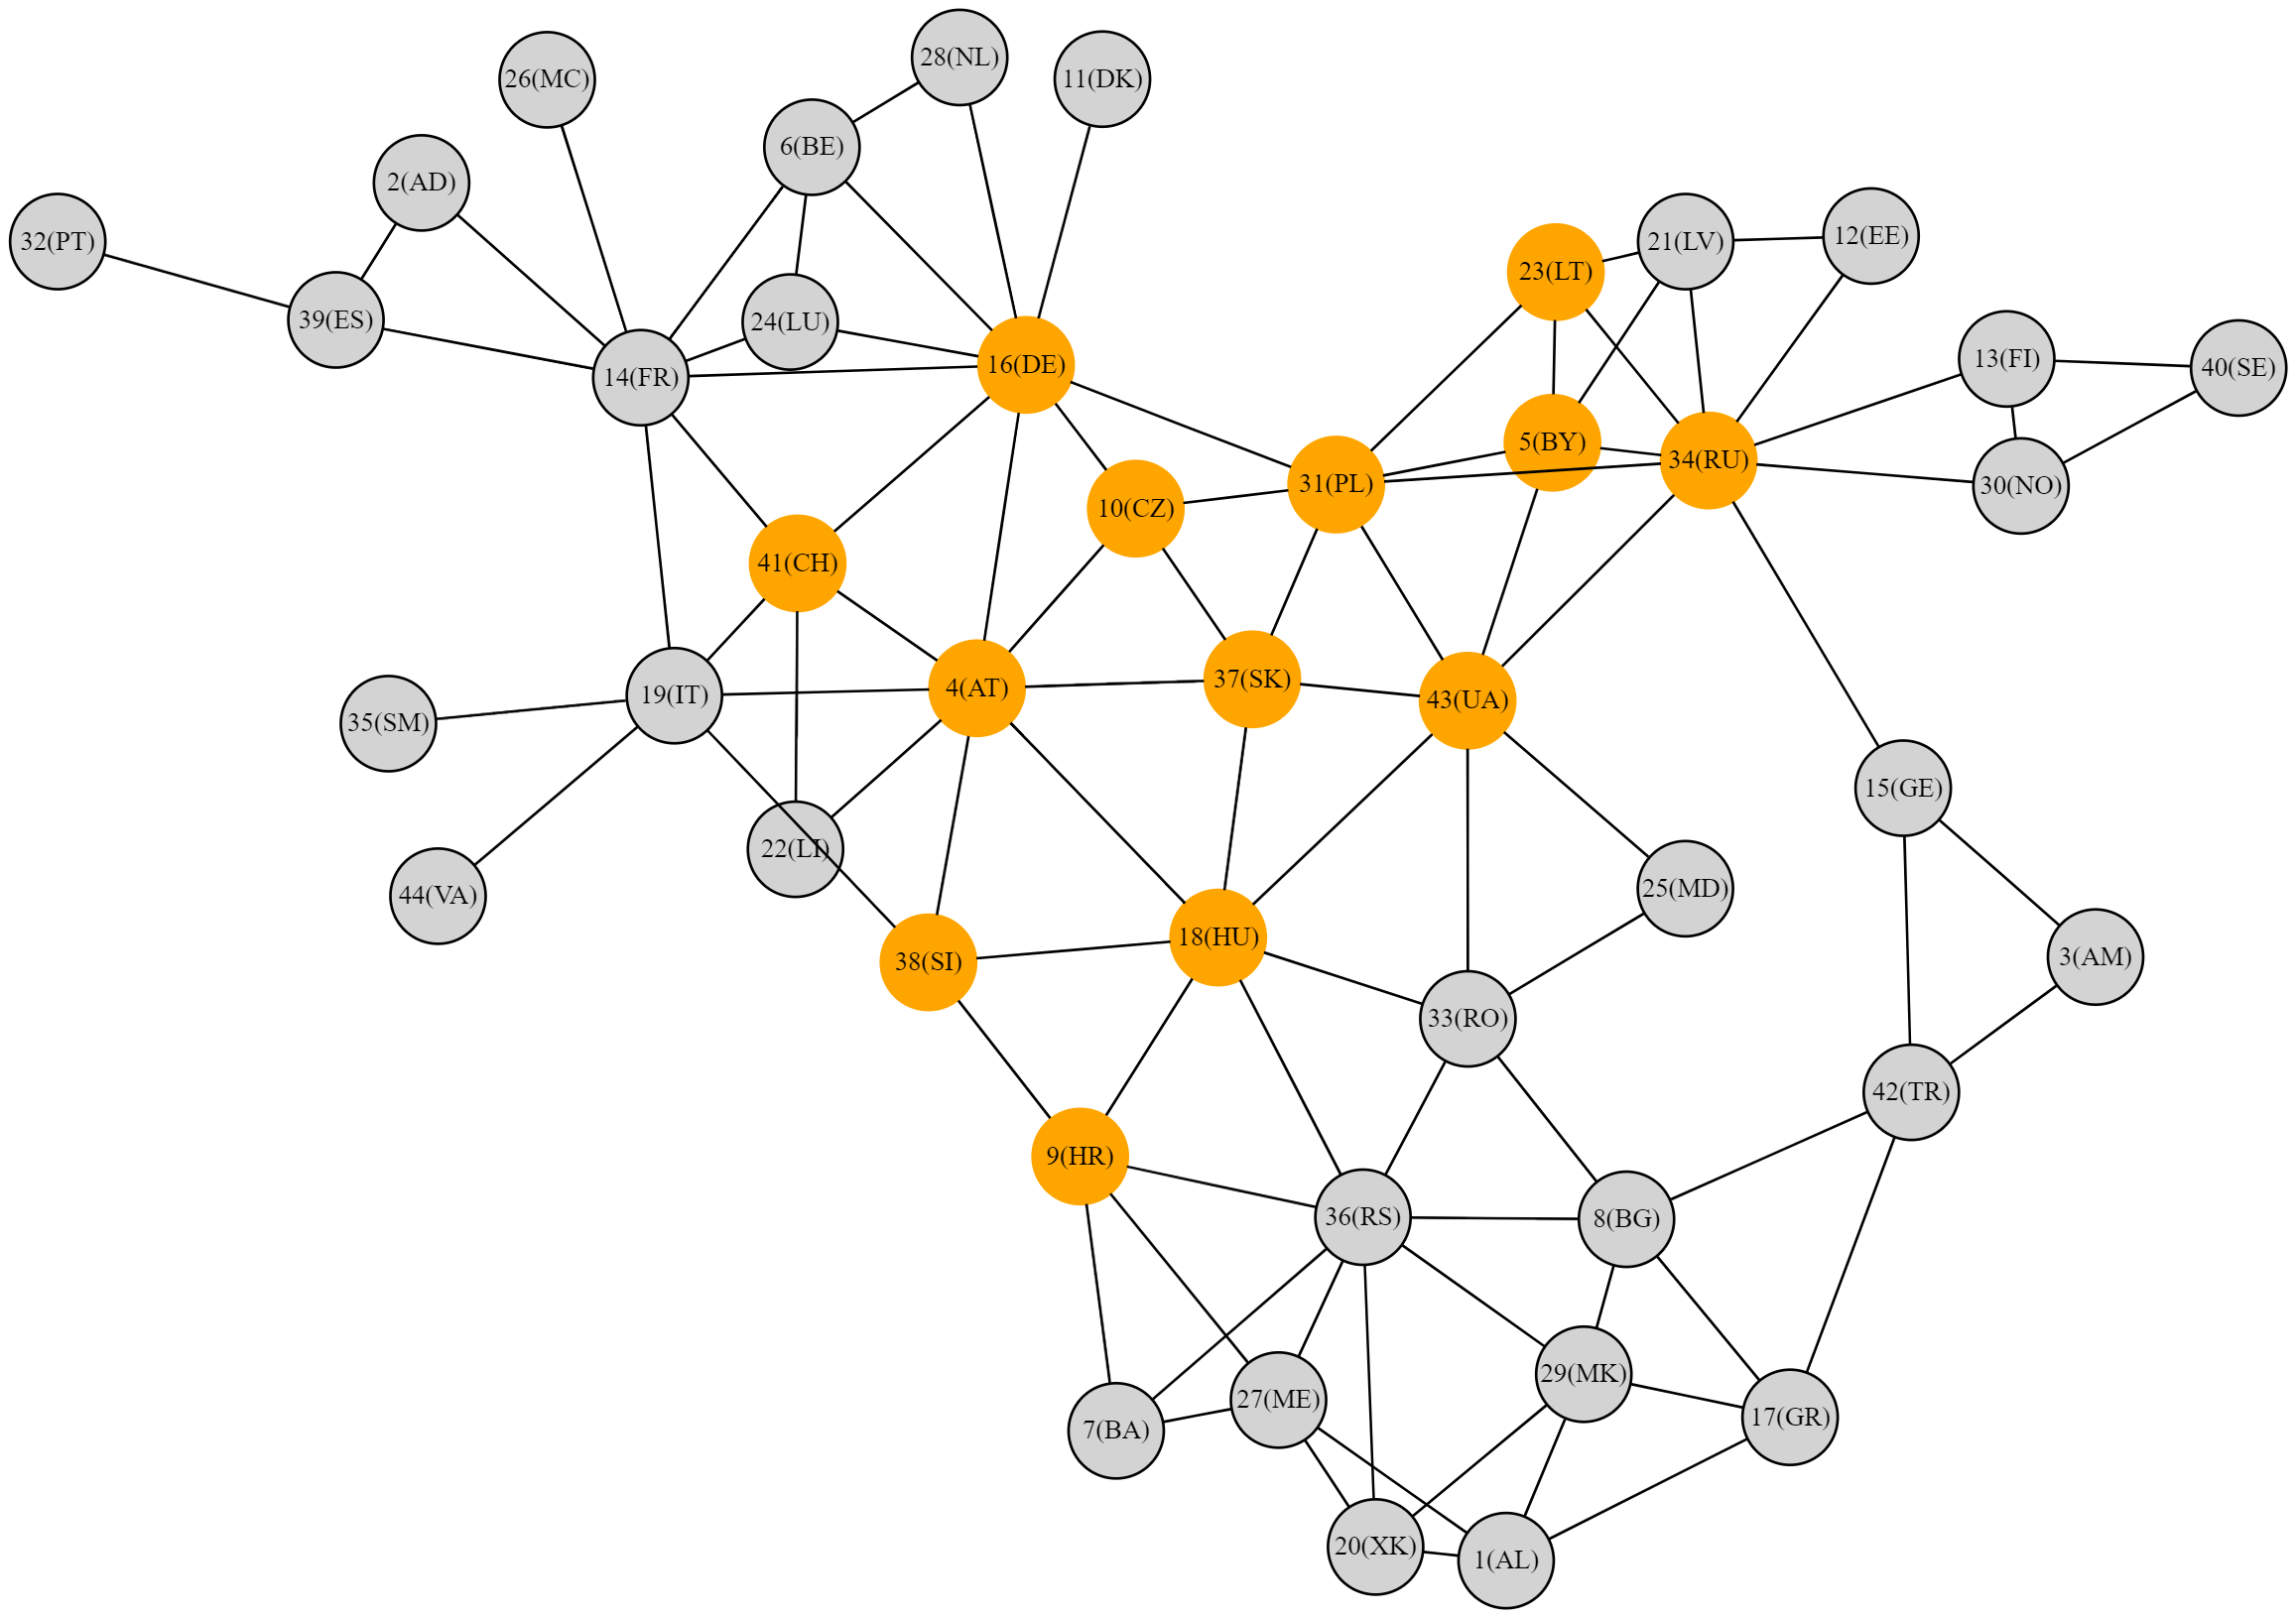
\includegraphics[width=1\textwidth]{center.png}
		\caption{center of $\mathcal{G}$ }
	\end{figure}\newpage
	(c), (d) It's easy to do these using MiniZinc. We just need to check that adjacent vertices (edges) don't have the same color and try to minimize number of colors. Number of vertex colors is 4 and the number of edge colors is 9.
	\begin{figure}[h]
		\centering
		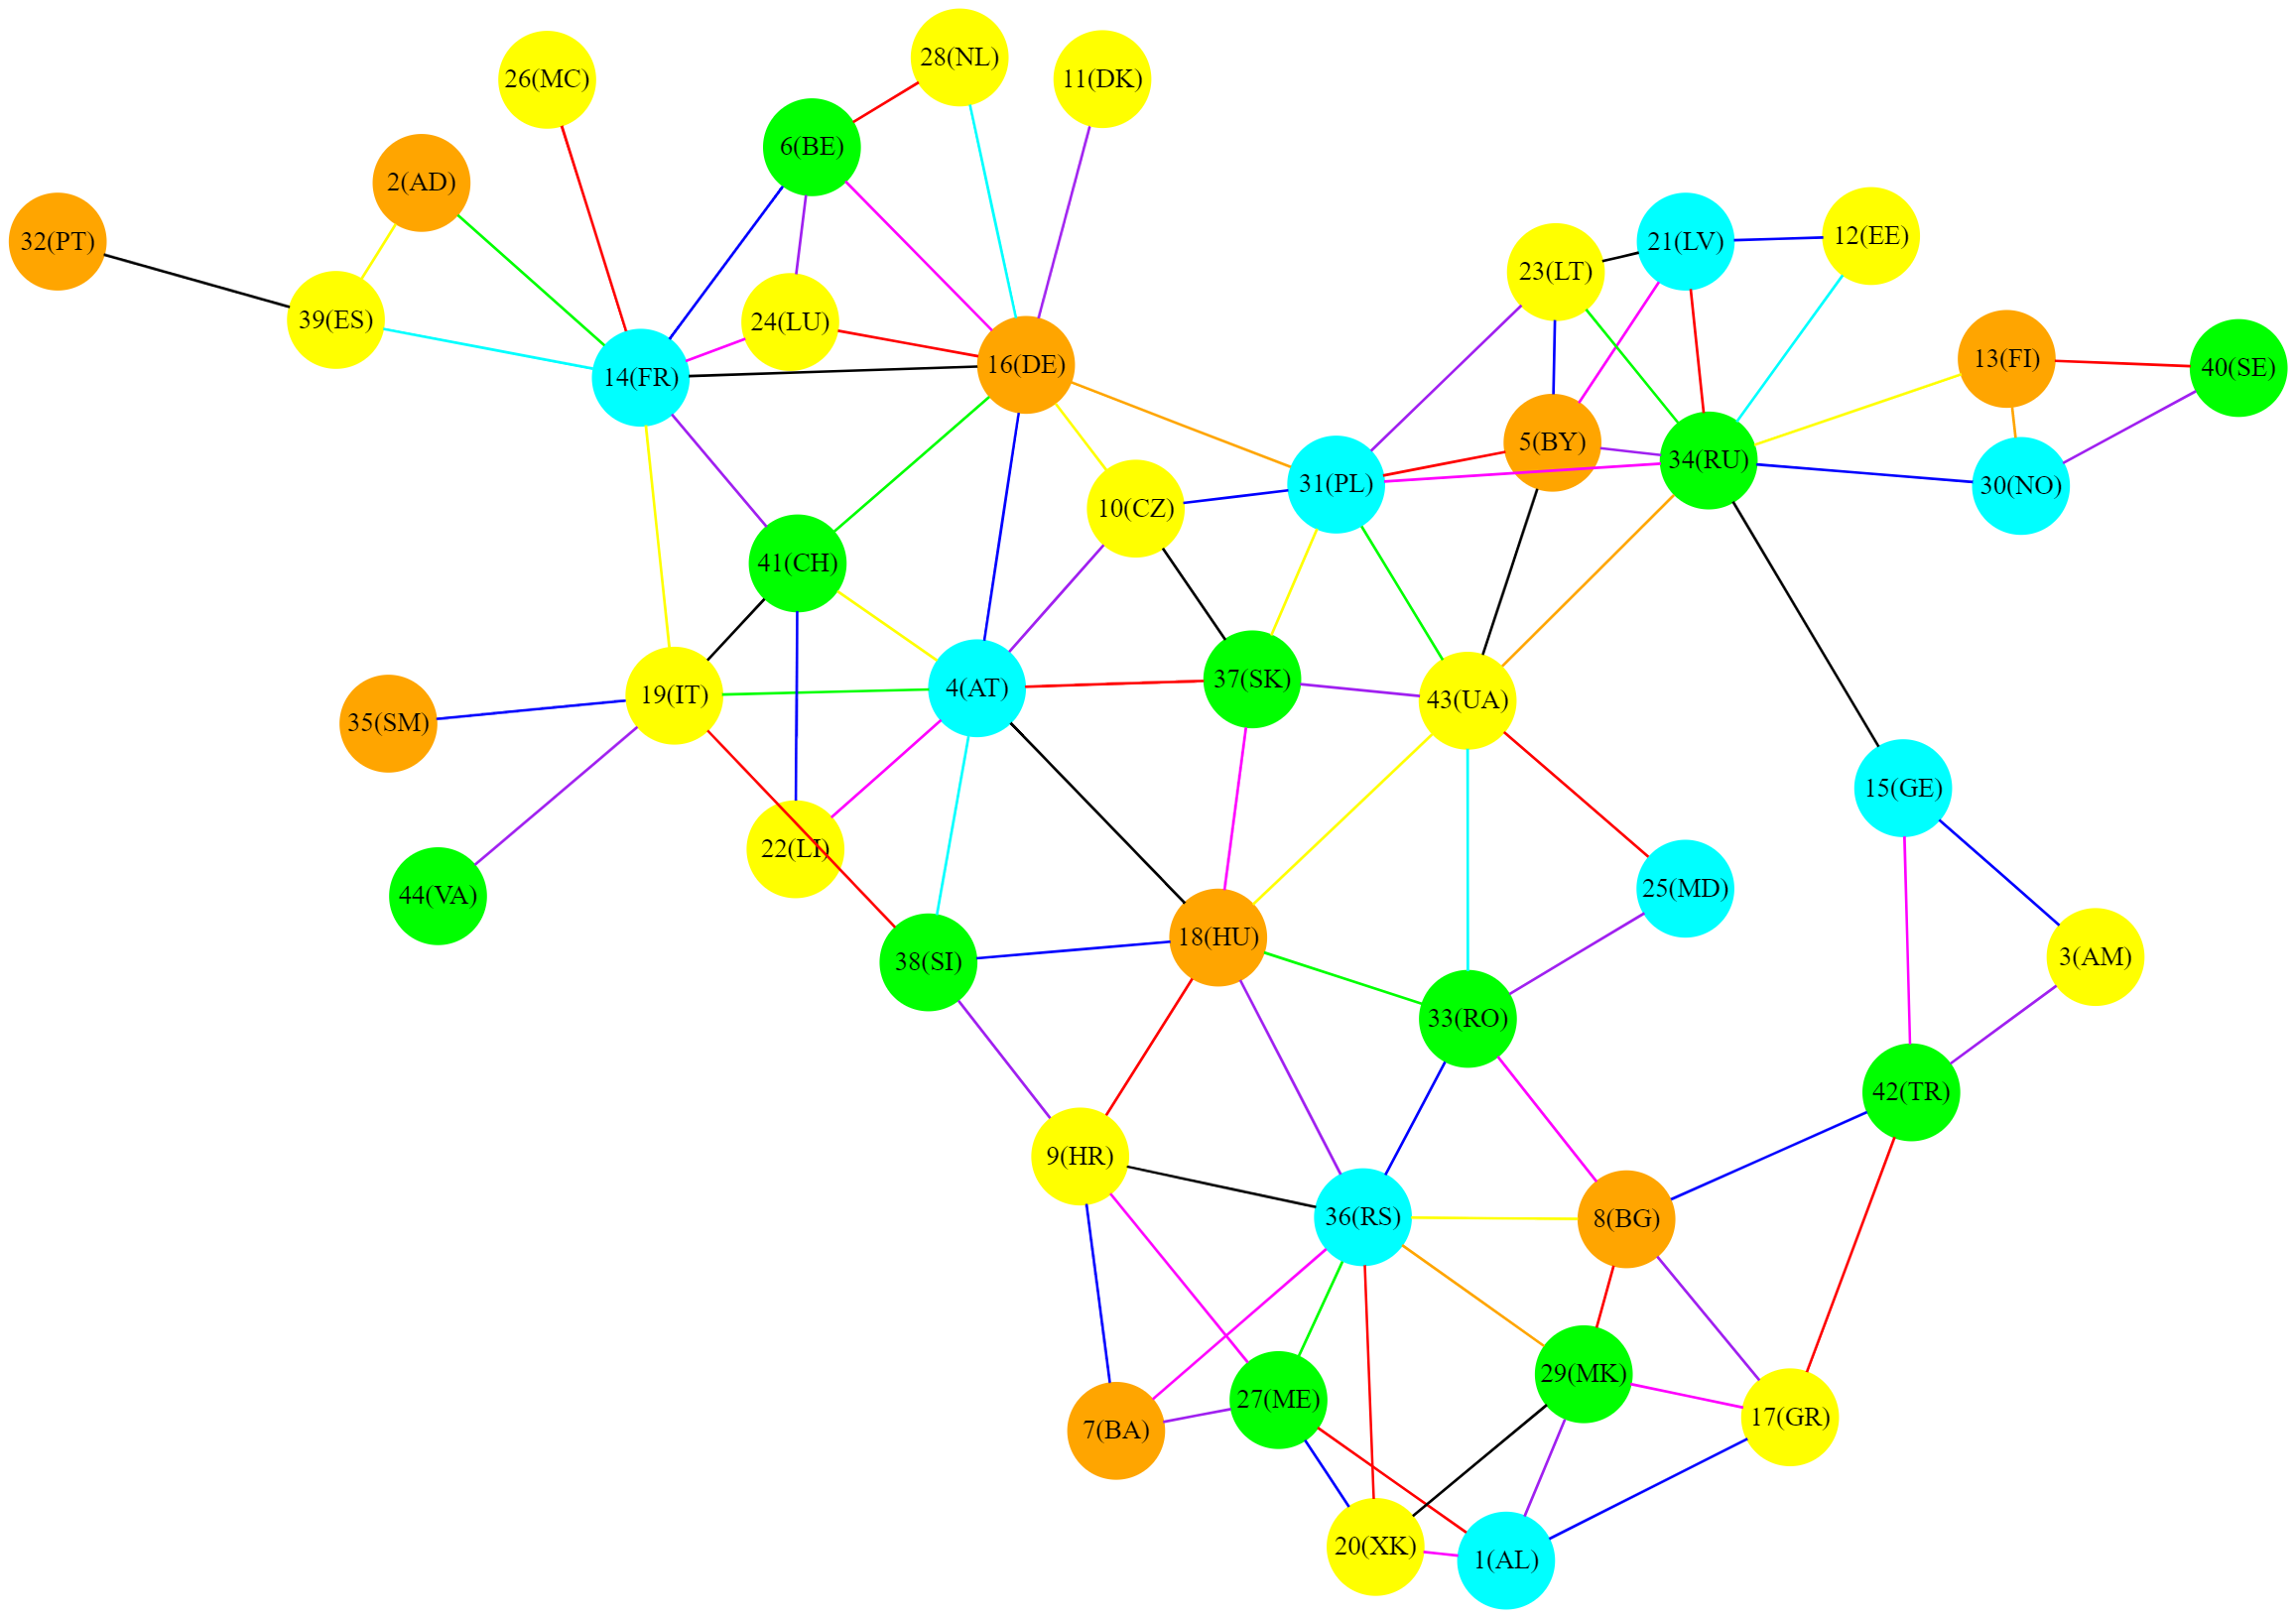
\includegraphics[width=1\textwidth]{v_e_coloring.png}
		\caption{vertex and edge colorings}
	\end{figure}\newpage
	(e) To find the maximum clique via MiniZinc we'll check that every pairwise distinct vertices in clique are adjacent. Size of such clique is 4.
	\begin{figure}[h]
		\centering
		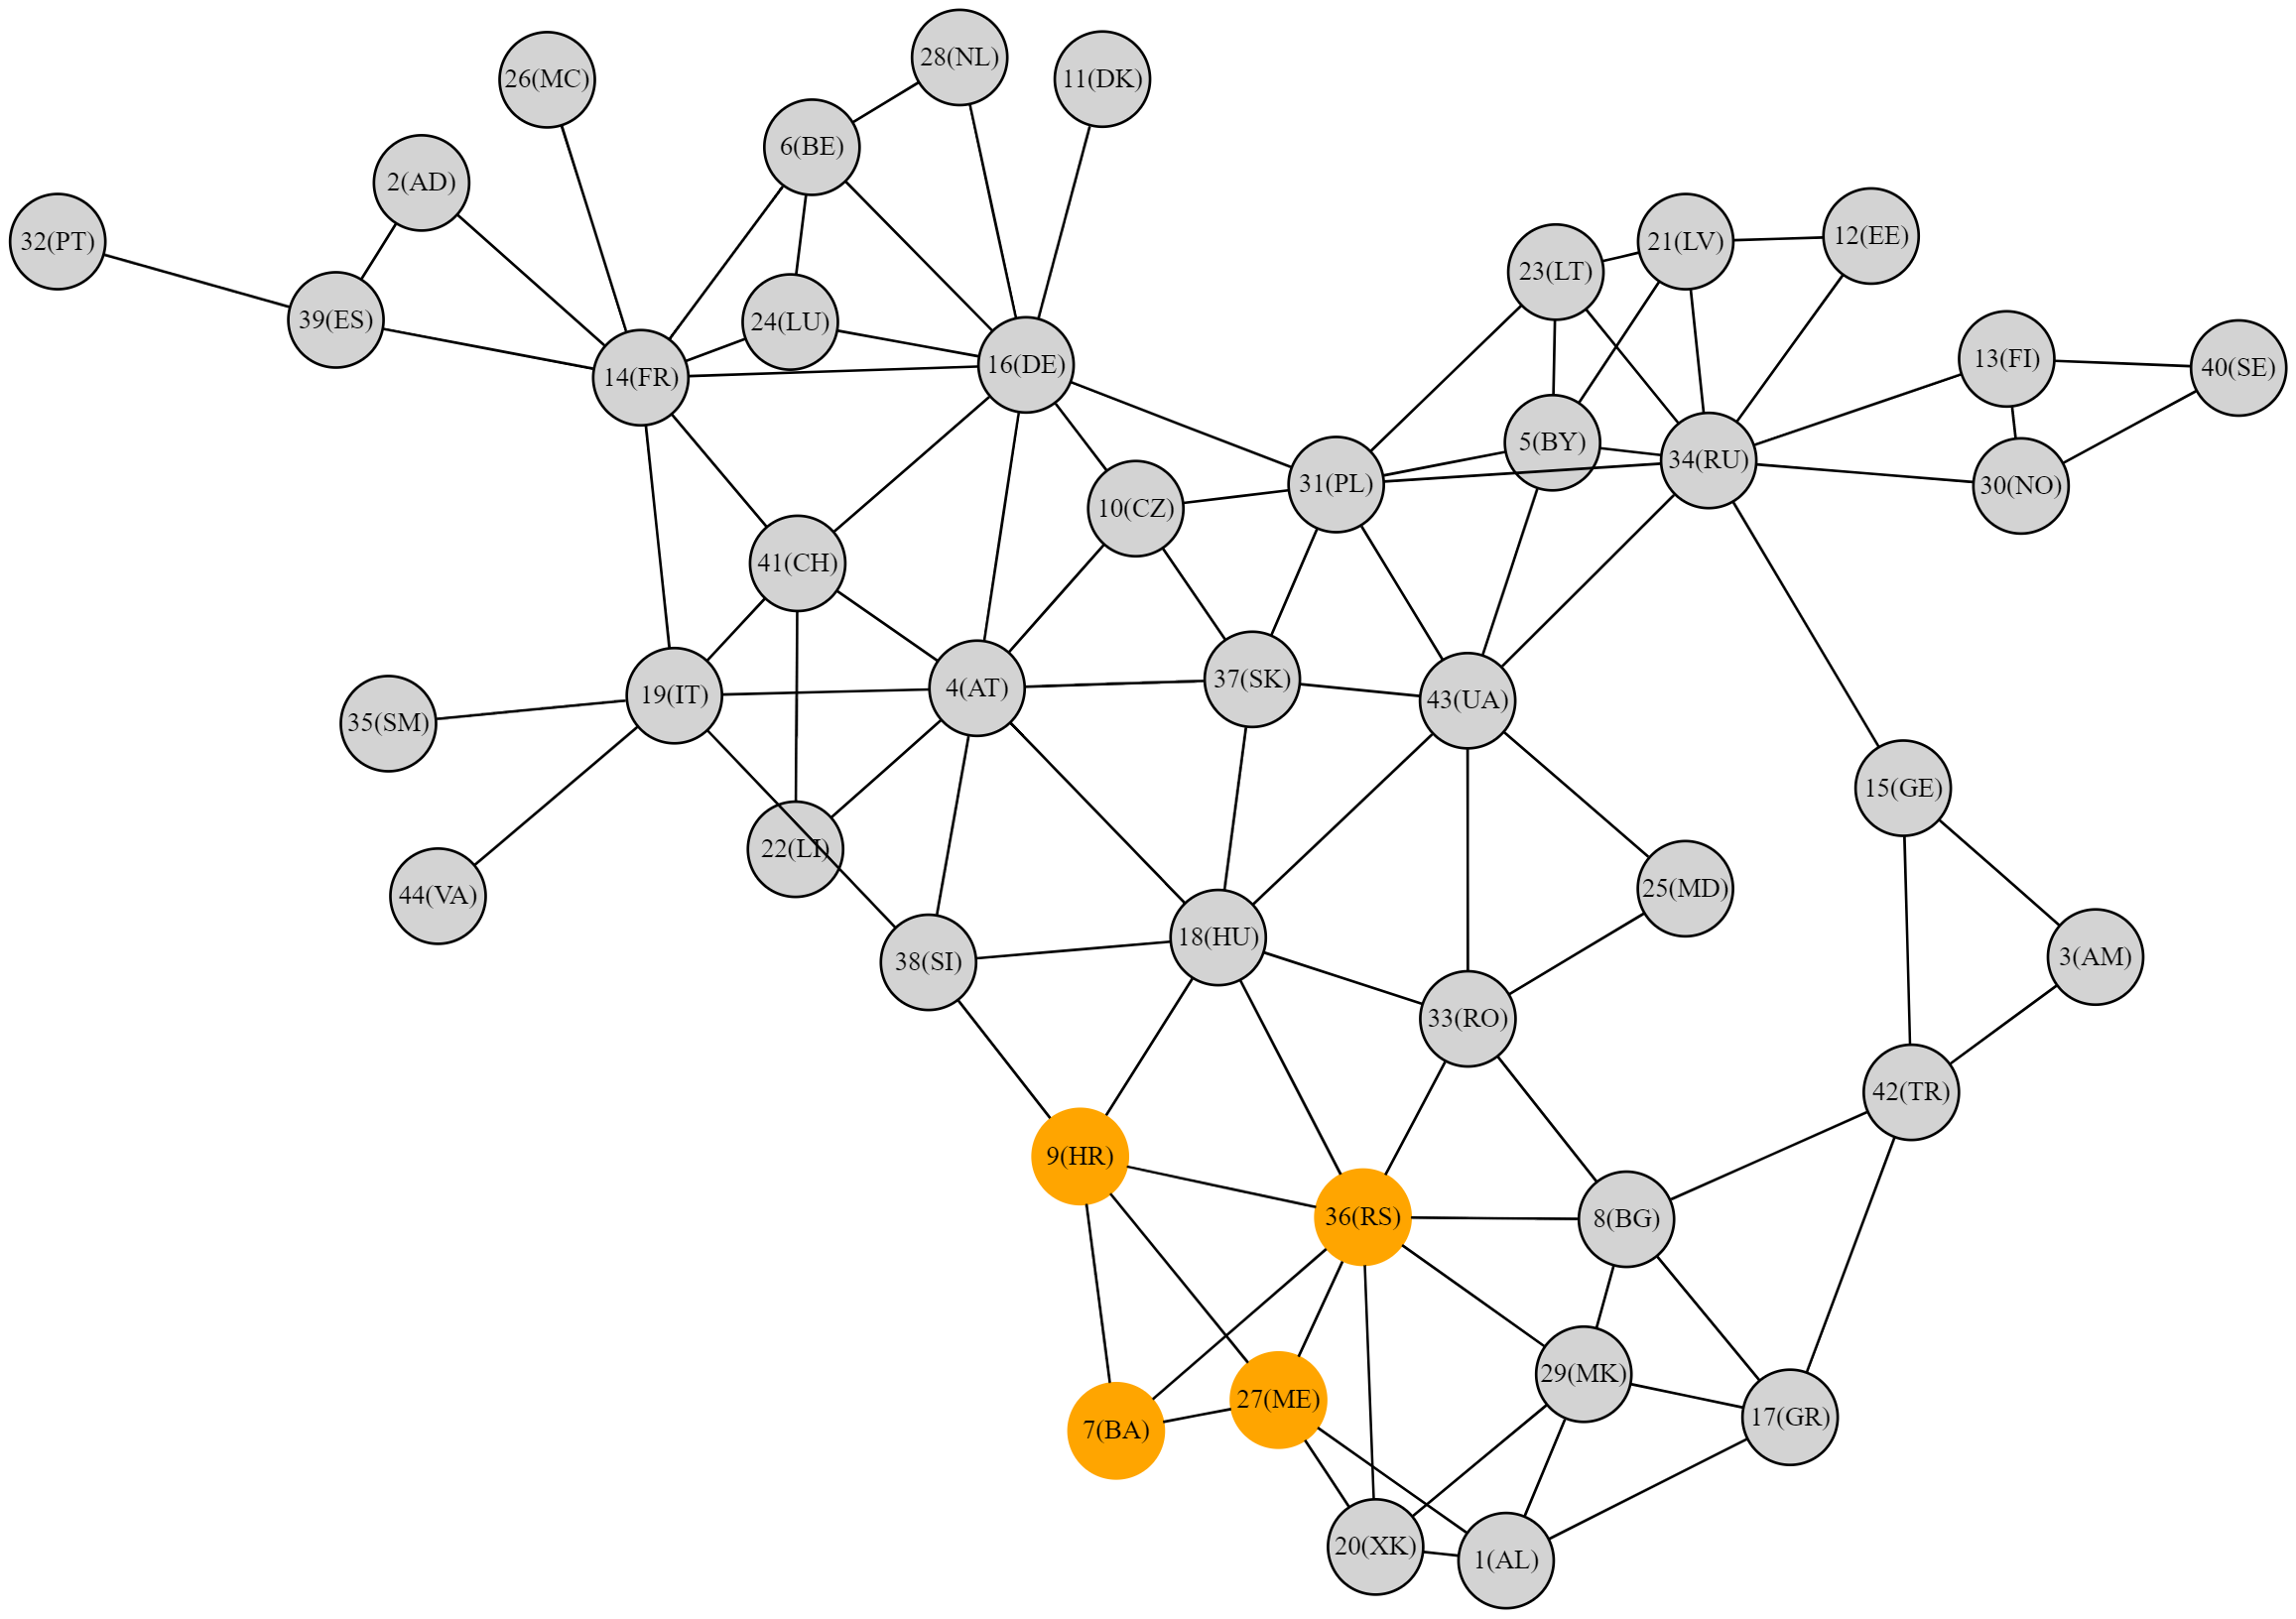
\includegraphics[width=1\textwidth]{clique.png}
		\caption{Maximum clique}
	\end{figure}\newpage
	(f) To find the maximum stable set via MiniZinc we'll check that vertices used in this set aren't adjacent. Size of such set is 19.
	\begin{figure}[h]
		\centering
		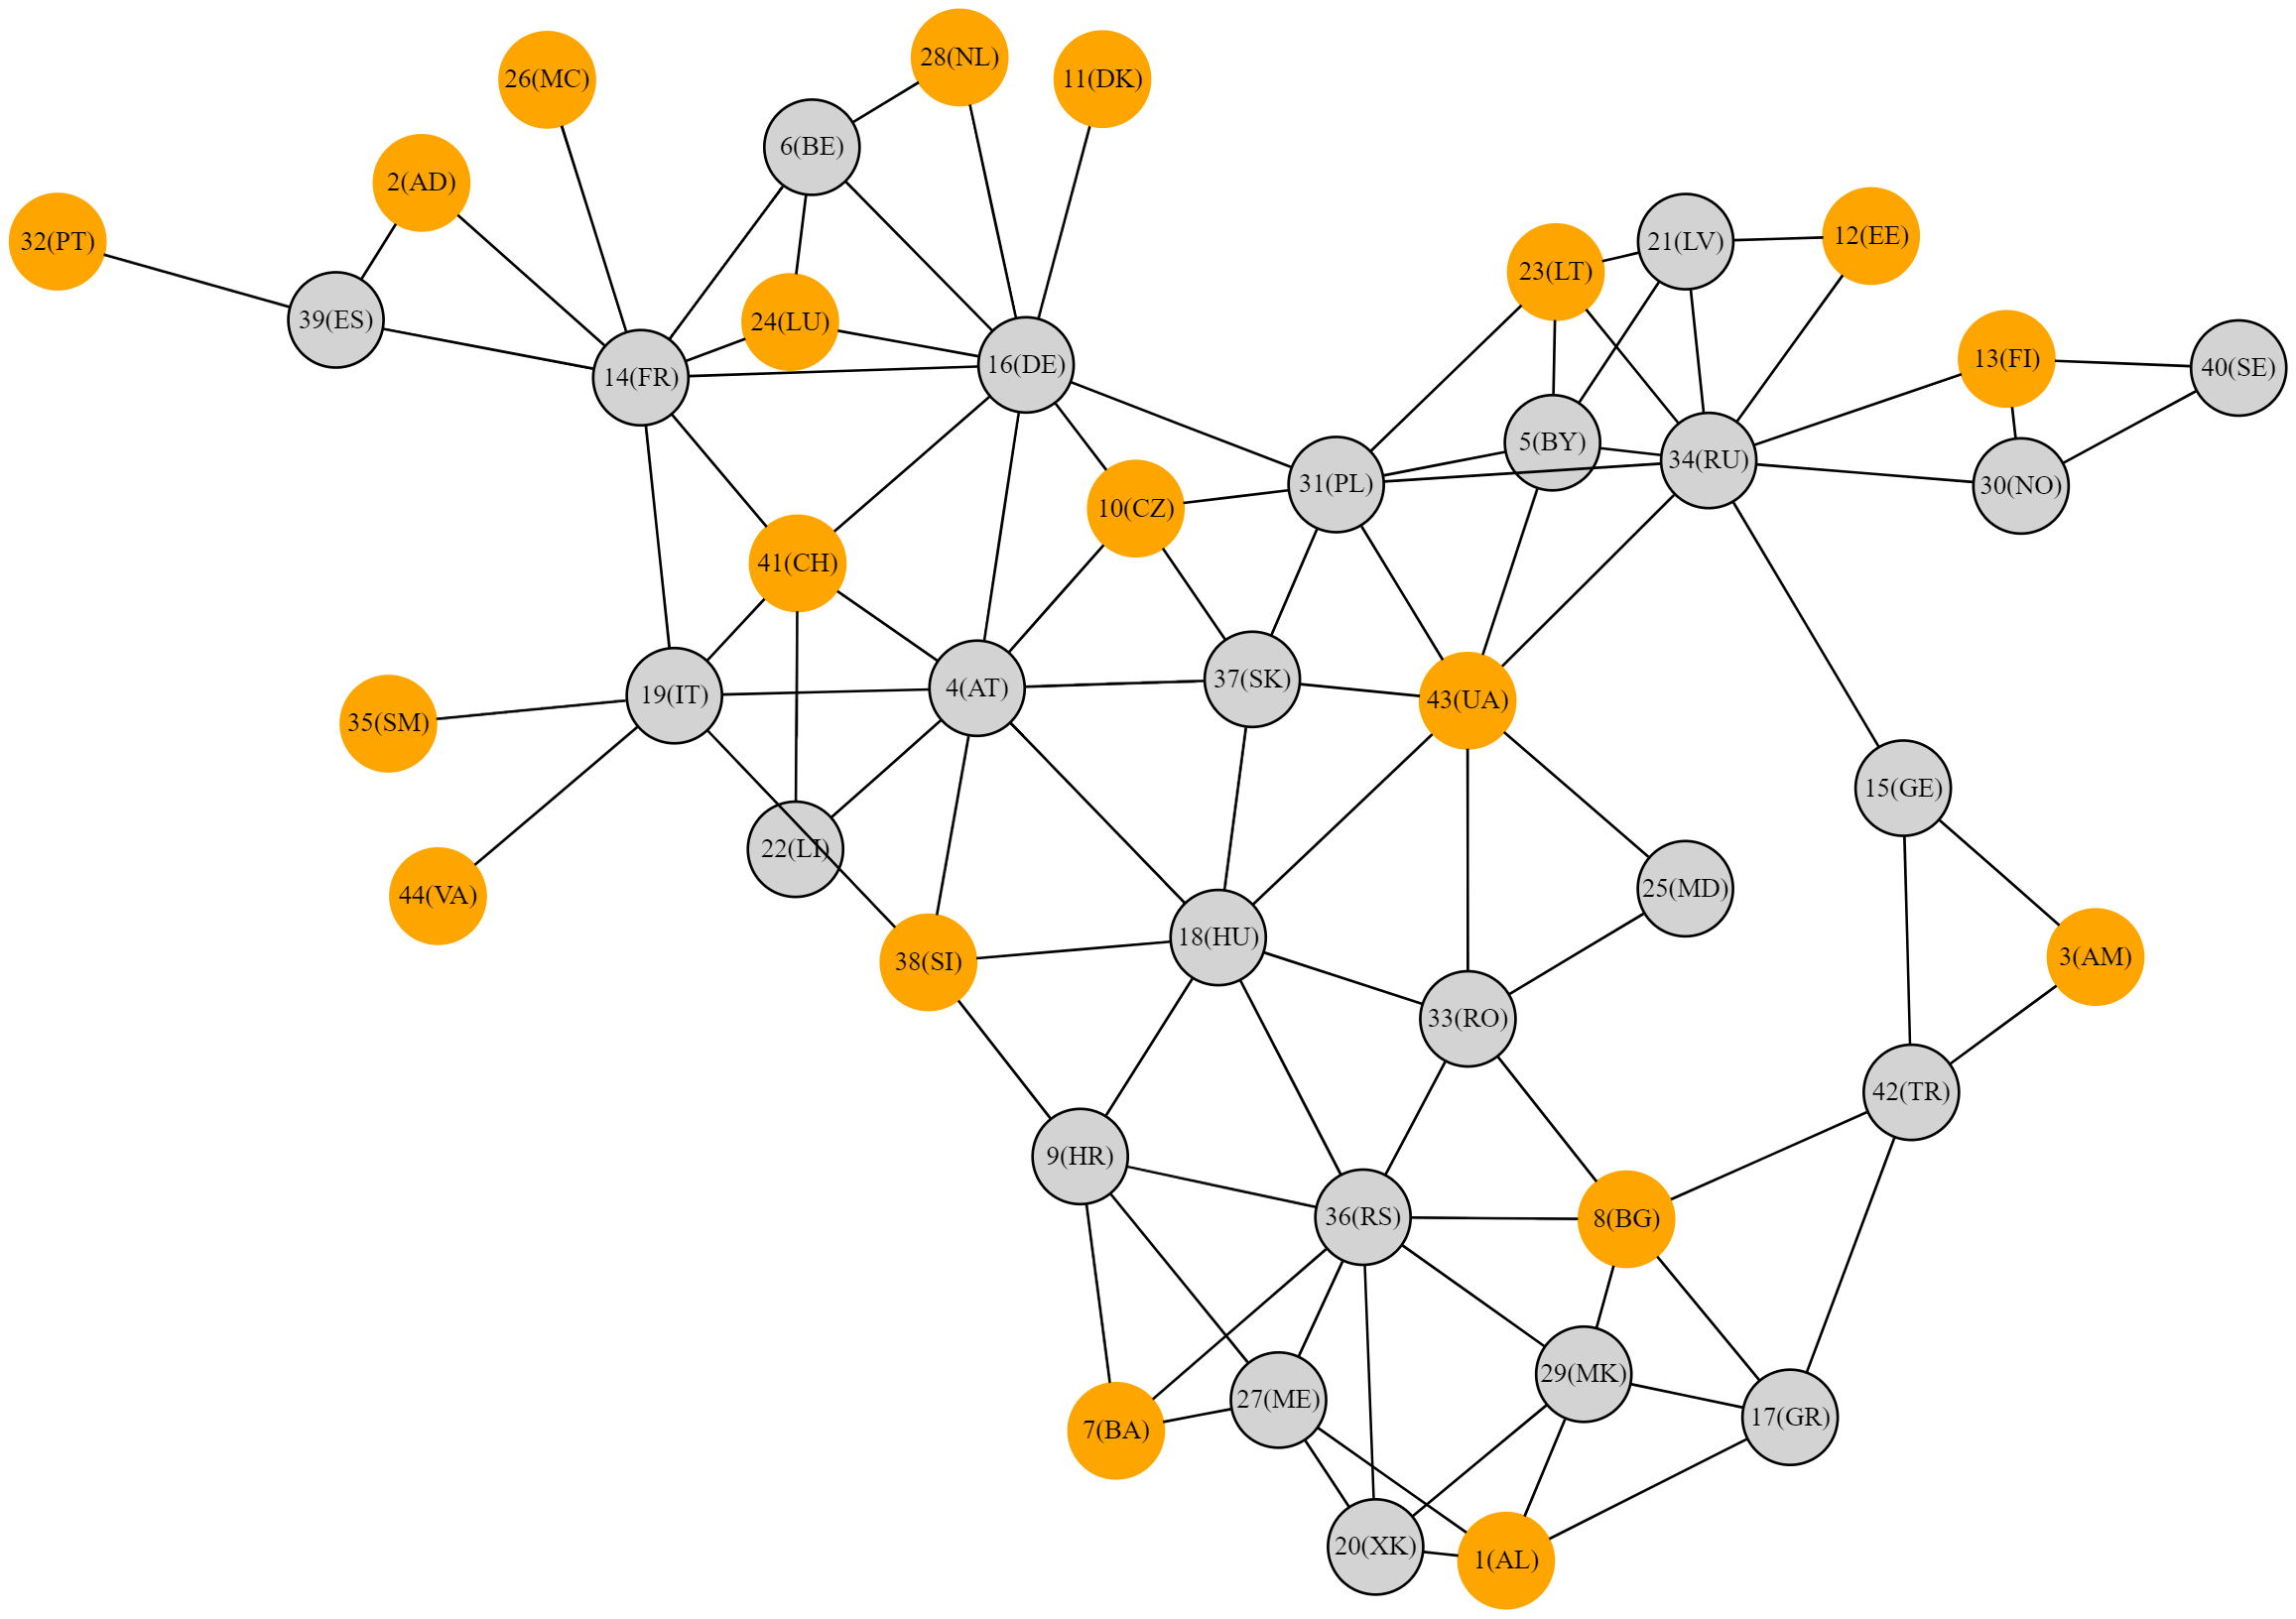
\includegraphics[width=1\textwidth]{stable set.png}
		\caption{Maximum stable set}
	\end{figure}\newpage
	(g) To find the maximum matching via MiniZinc we'll check that edges used in this set aren't adjacent. Size of such matching is 20.
	\begin{figure}[h]
		\centering
		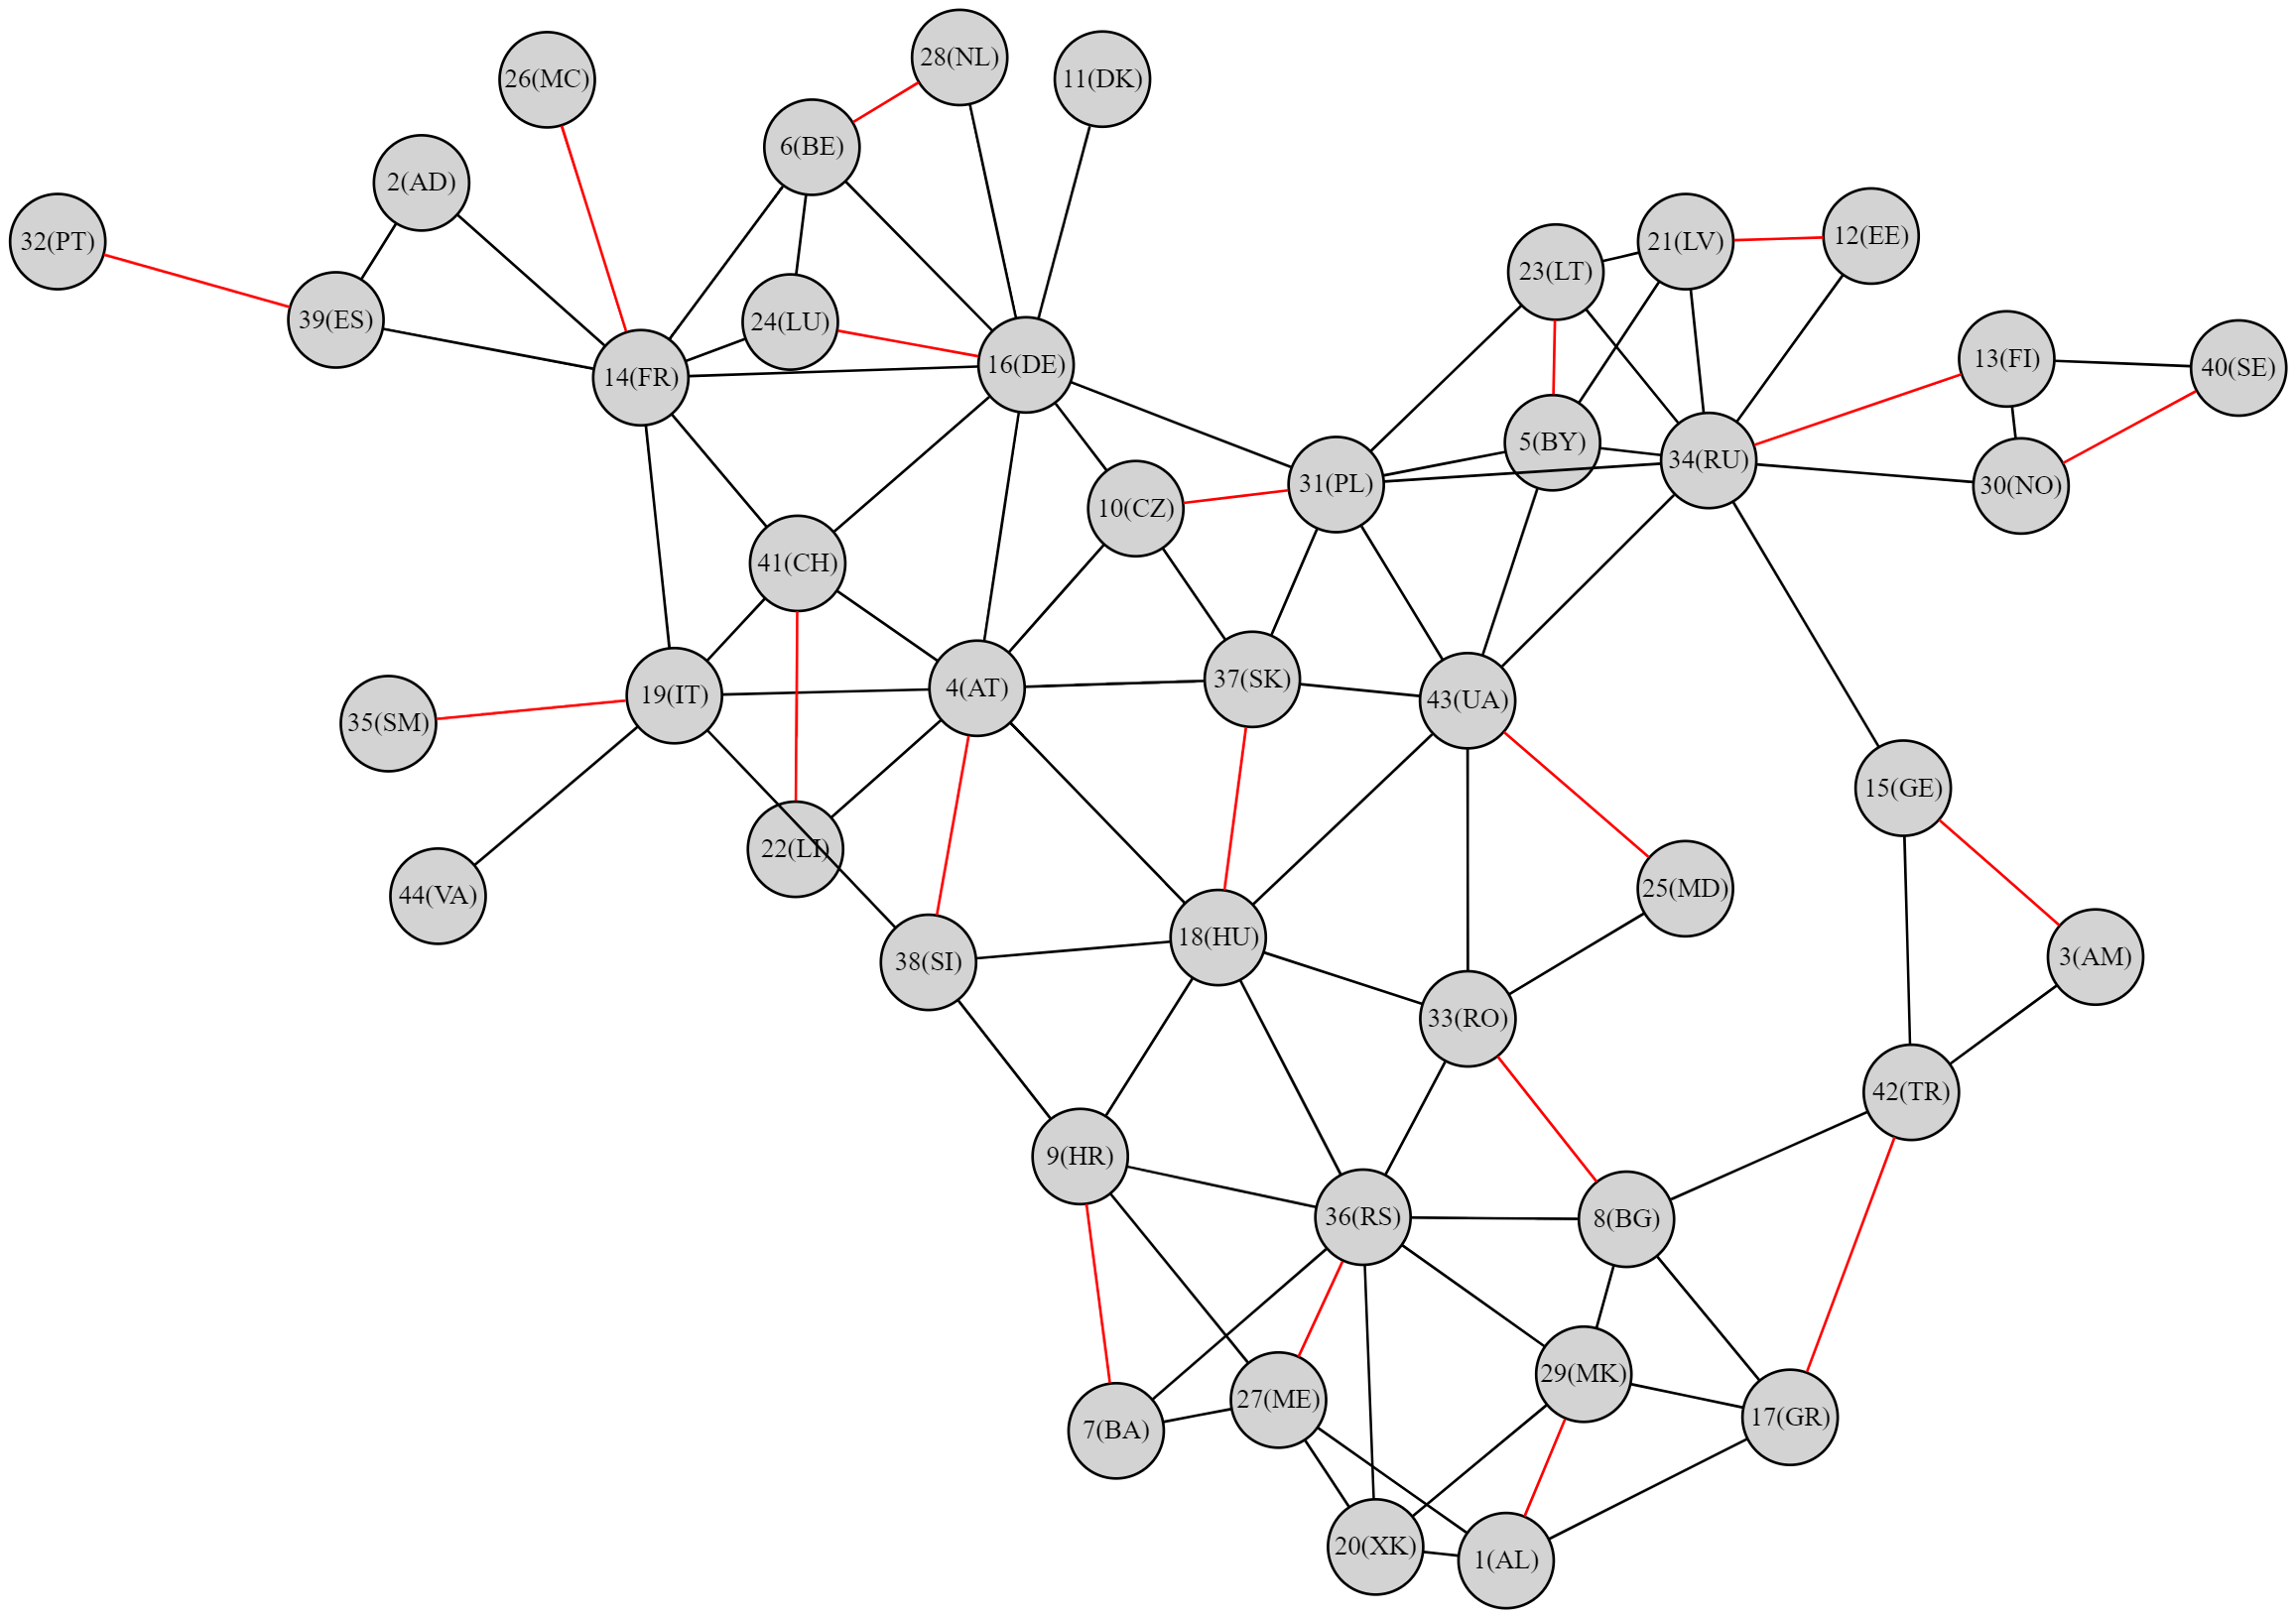
\includegraphics[width=1\textwidth]{matching.png}
		\caption{Maximum matching}
	\end{figure}\newpage
	(h) To find the minimum vertex cover via MiniZinc we'll check that for every edje in the graph at least one of its incident vertives is in this set. Size of such set is 25.
	\begin{figure}[h]
		\centering
		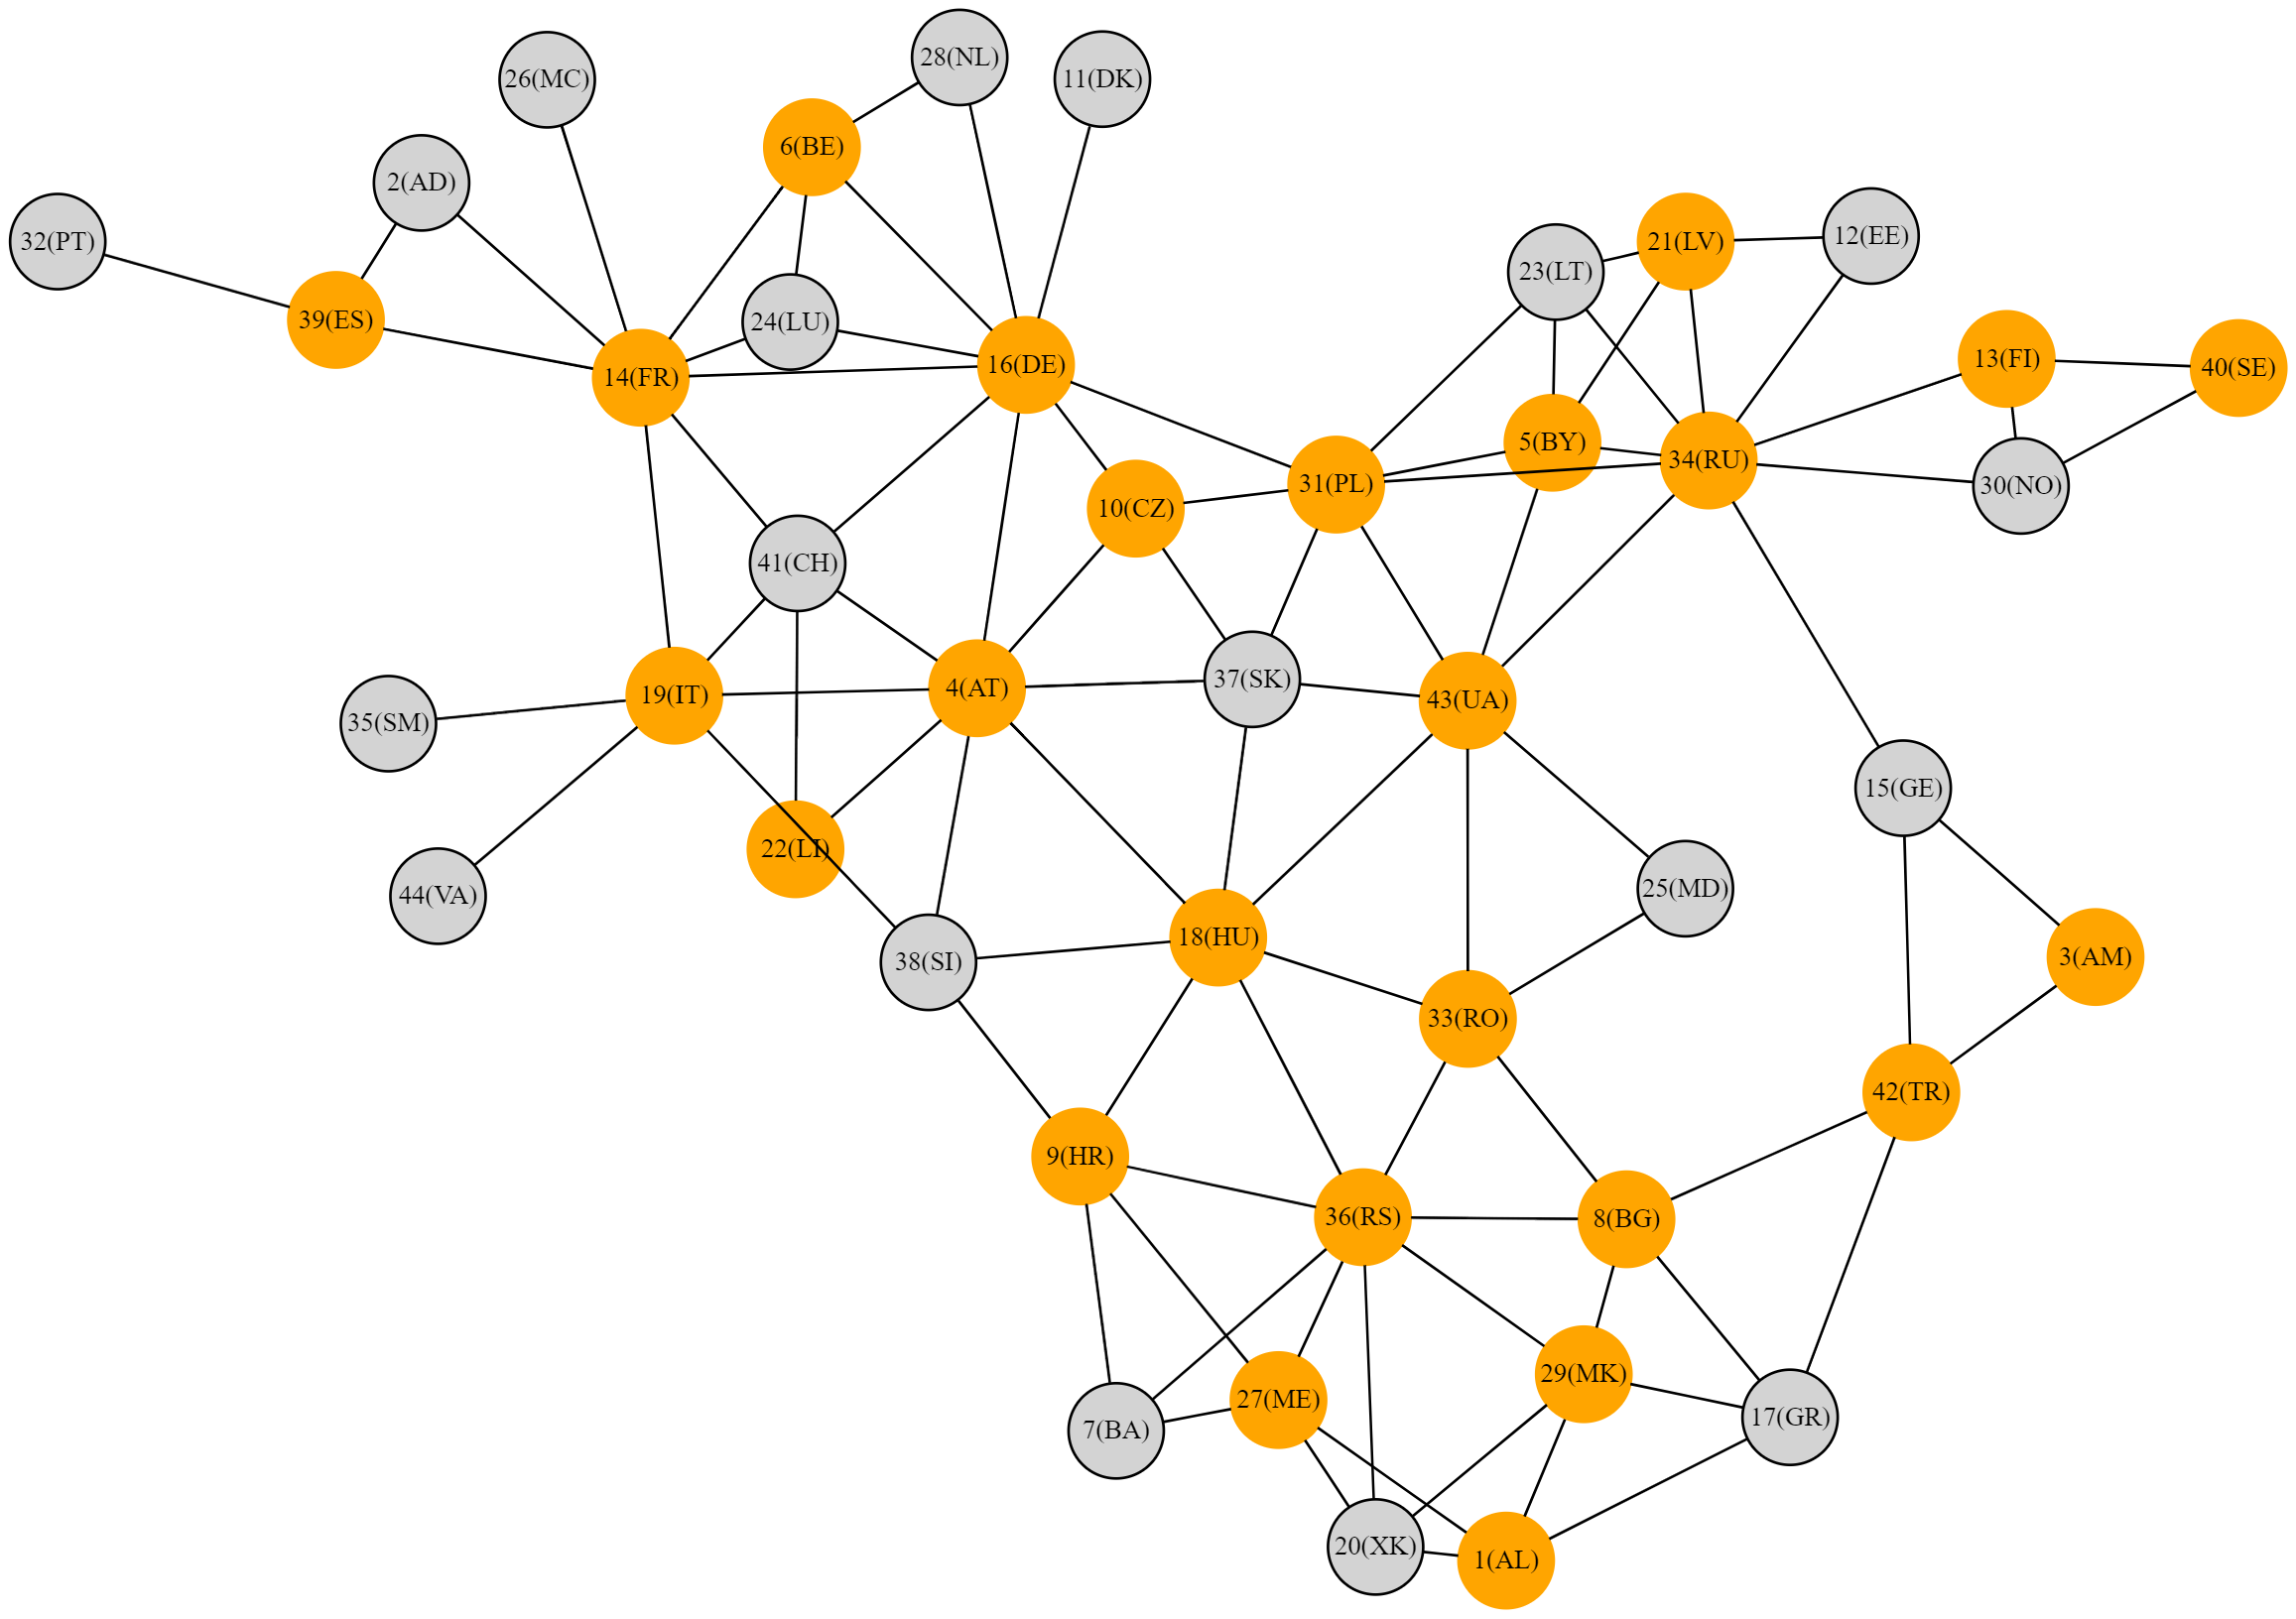
\includegraphics[width=1\textwidth]{v_cover.png}
		\caption{Minimum vertex cover}
	\end{figure}\newpage
	(i) To find the minimum edge cover via MiniZinc we'll check that every vertex in the graph is incident to at least 1 edge from this set. Size of such set is 24.
	\begin{figure}[h]
		\centering
		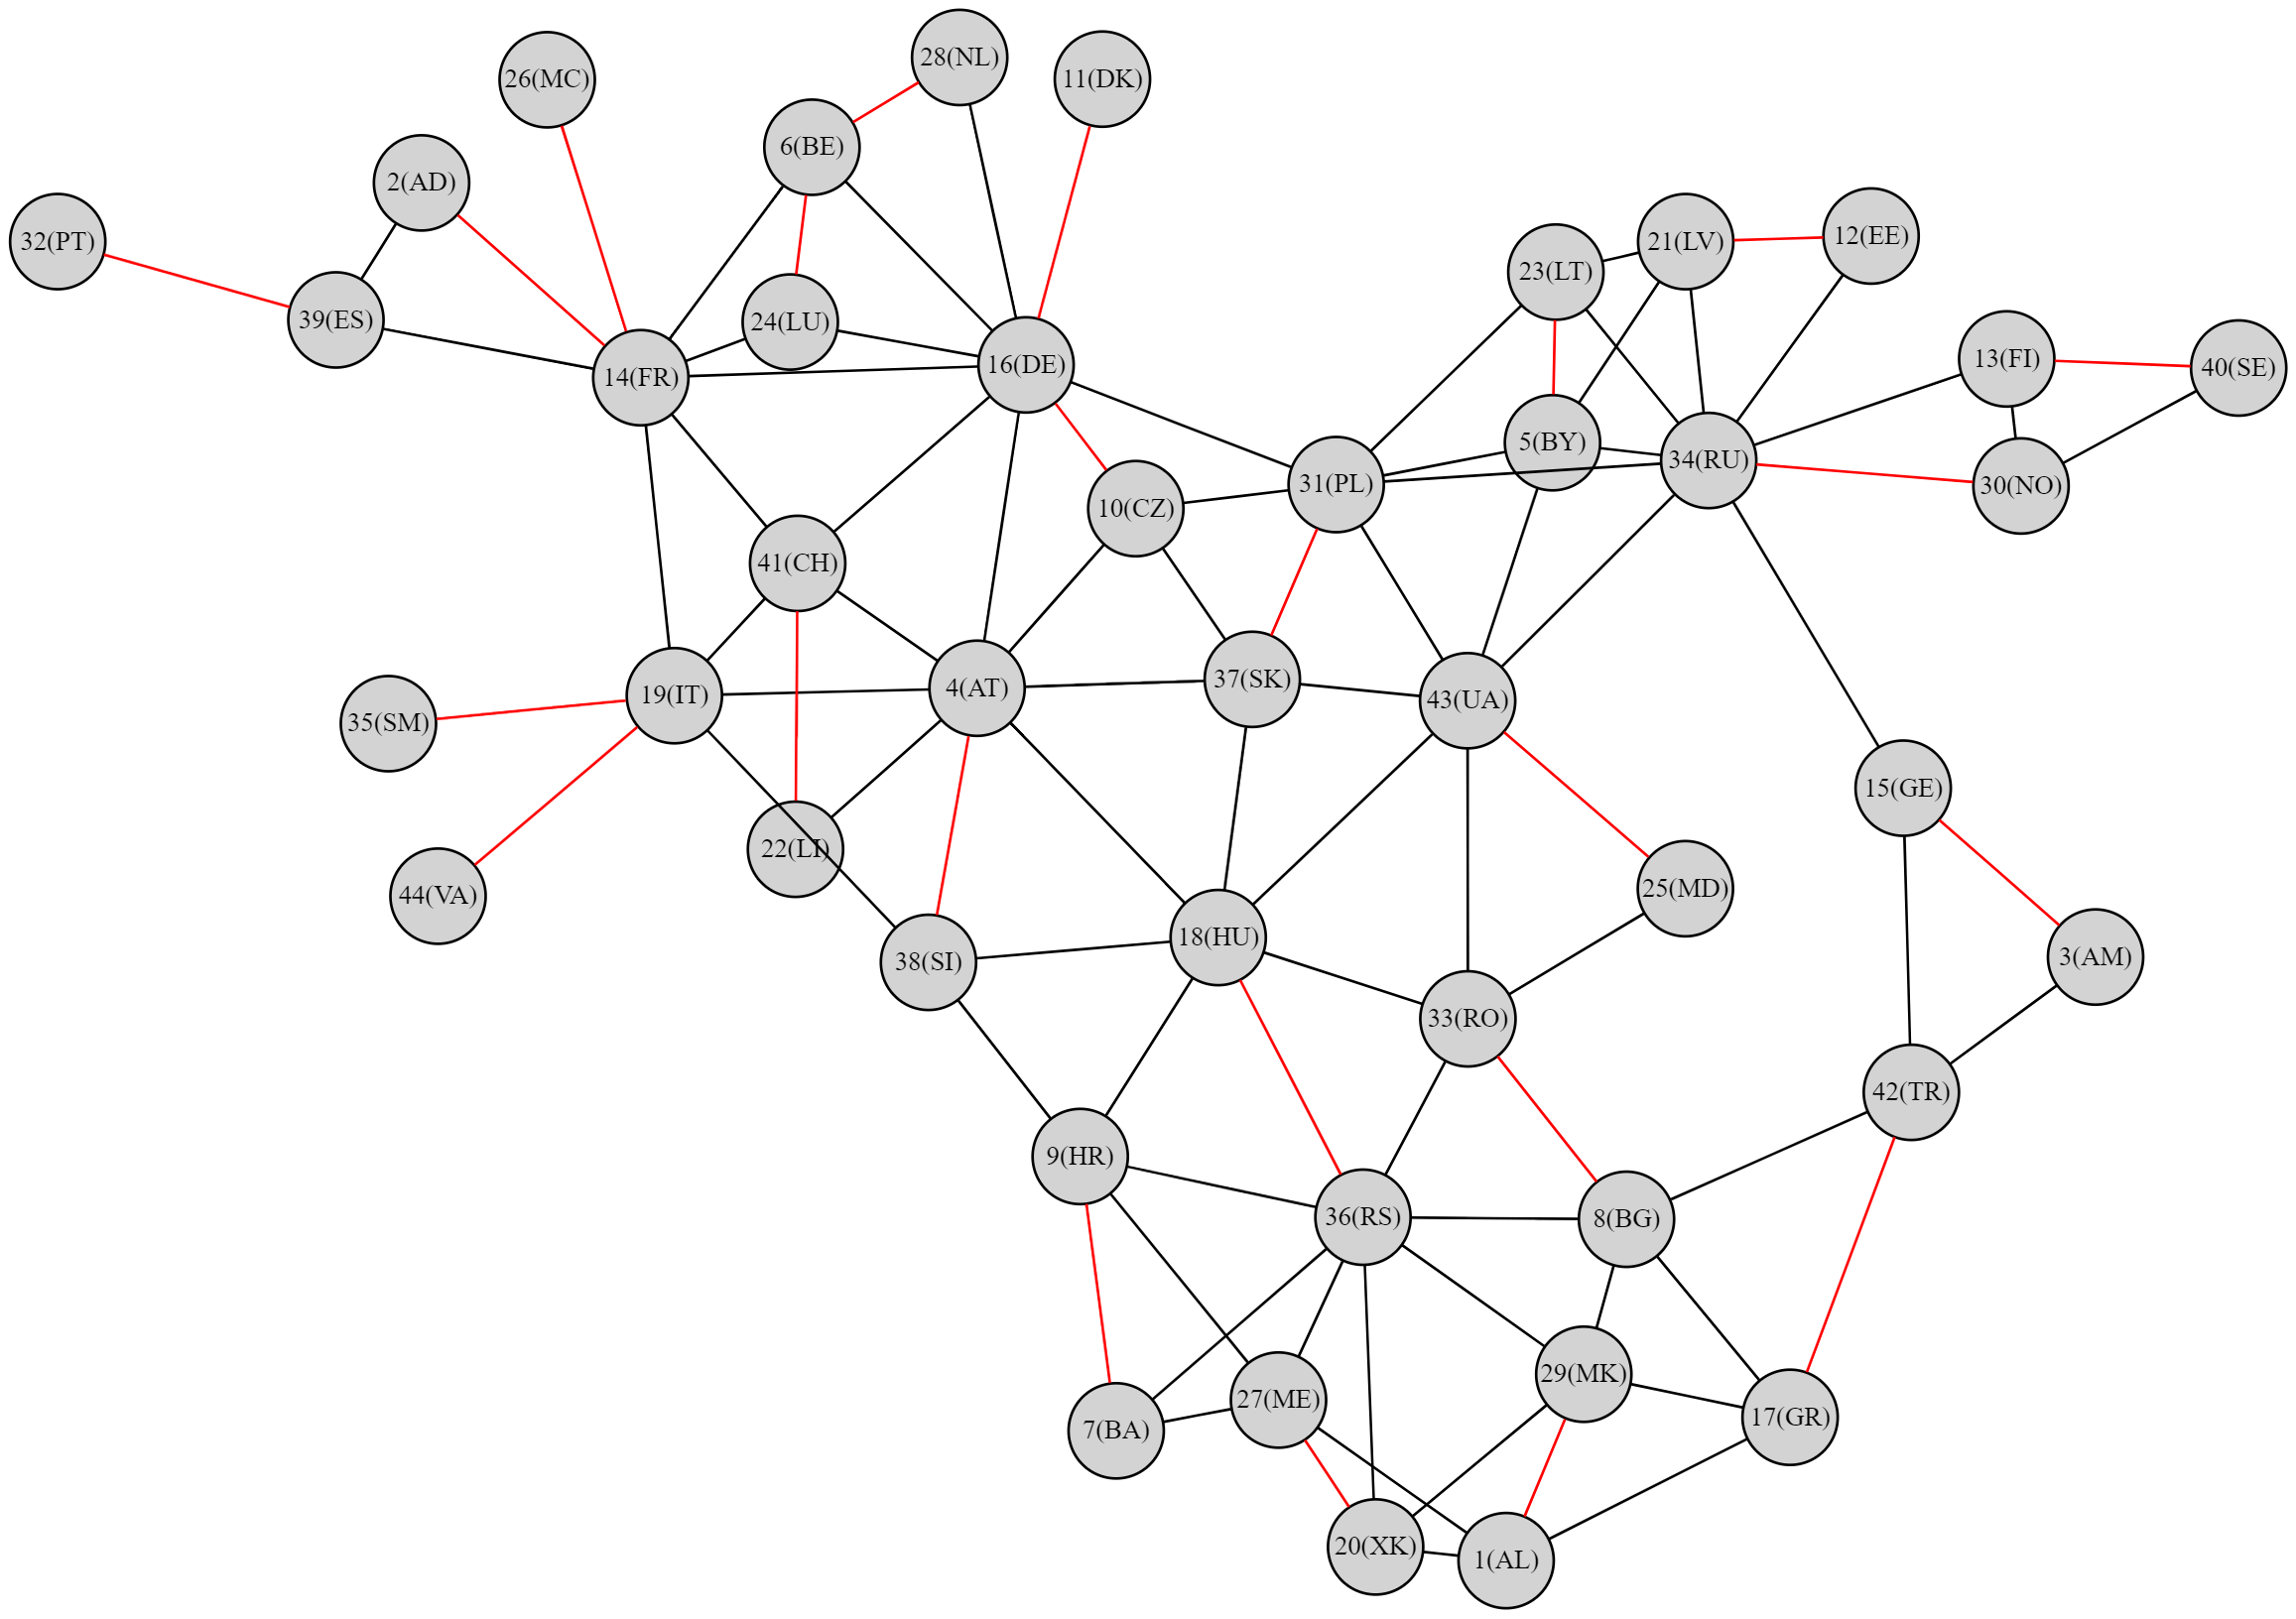
\includegraphics[width=1\textwidth]{ecover.png}
		\caption{Minimum edge cover}
	\end{figure}\newpage
	(j) At first we'll consider subgraph of $\mathcal{G}$, induced on all vertices except those which are highlighted in blue. In such subgraph we can find Hamiltonian cycle of size 34 -- its edges are highlighted in red. It's impossible to add blue vertices to this cycle in $\mathcal{G}$ to make it Hamiltonian in $\mathcal{G}$ because they're connected to subgraph only by cut vertices. We can still add purple edges to the cycle to make from it the walk that visits all vertices. We have to use IT-SM, IT-VA, FR-MC, DE-DK, ES-PT twice as they're bridges. To add other blue vertices we need $3 + 4 = 7$ more edges (it's easy to find shortest walks in these little subgraphs -- we have few edges to search through). So the length of the shortest walk that visits all vertices is 51.
	\begin{figure}[h]
		\centering
		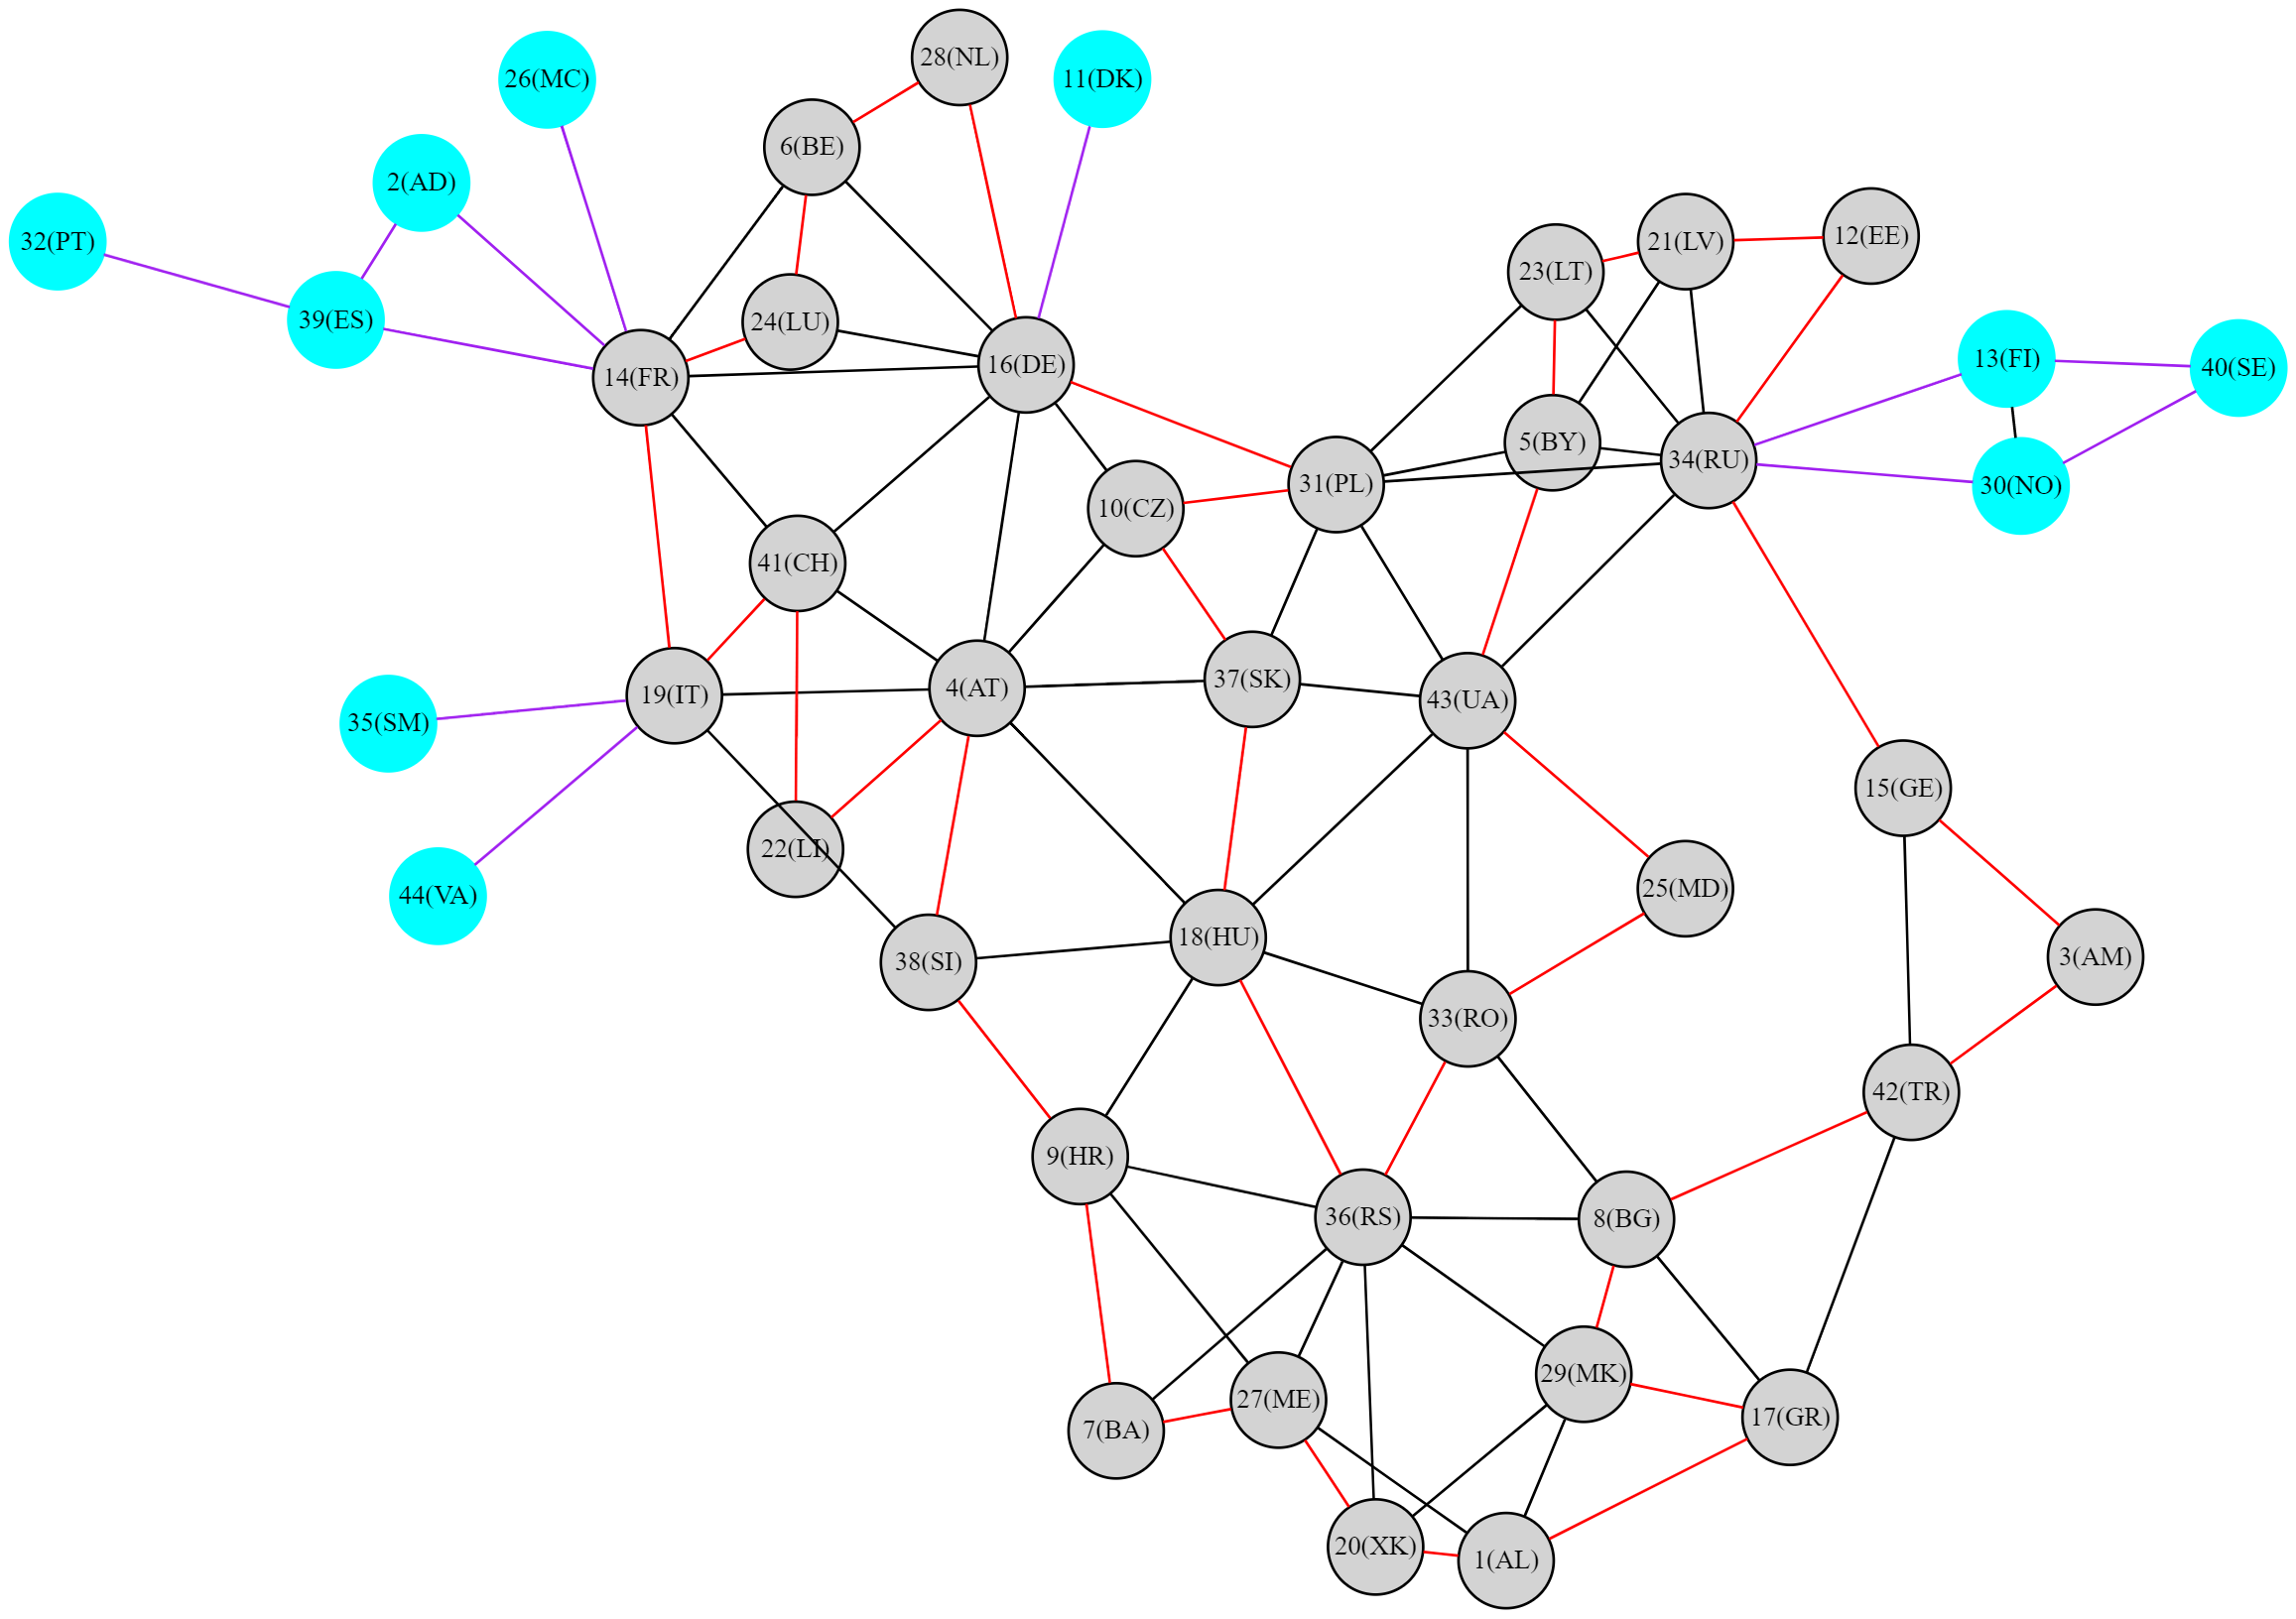
\includegraphics[width=1\textwidth]{v_walk.png}
		\caption{Shortest 'vertex' walk}
	\end{figure}\newpage
	(k)\newpage
	(l) Here we'll consider biconnectivity relation as relation on $E^2$, where the edges of a block belong to one equivalence class if subgraph on them and their incident vertices is maximal 2-vertex-connected or it's $K_2$ and doesn't belong to 2-vertex-connected subgraph. Then all we need to do is manually find cut vertices for each connected component and split connected components into blocks (blocks share no or only cut vertices). There are a total of 9 blocks here. \\\\
	As one block is disconnected from the graph it is only possible to draw separated block-cut trees. Block-cut tree of GB-IE block is $K_1$, so it makes sense to draw block-cut tree of $\mathcal{G}$.
	\begin{figure}[h]
		\centering
		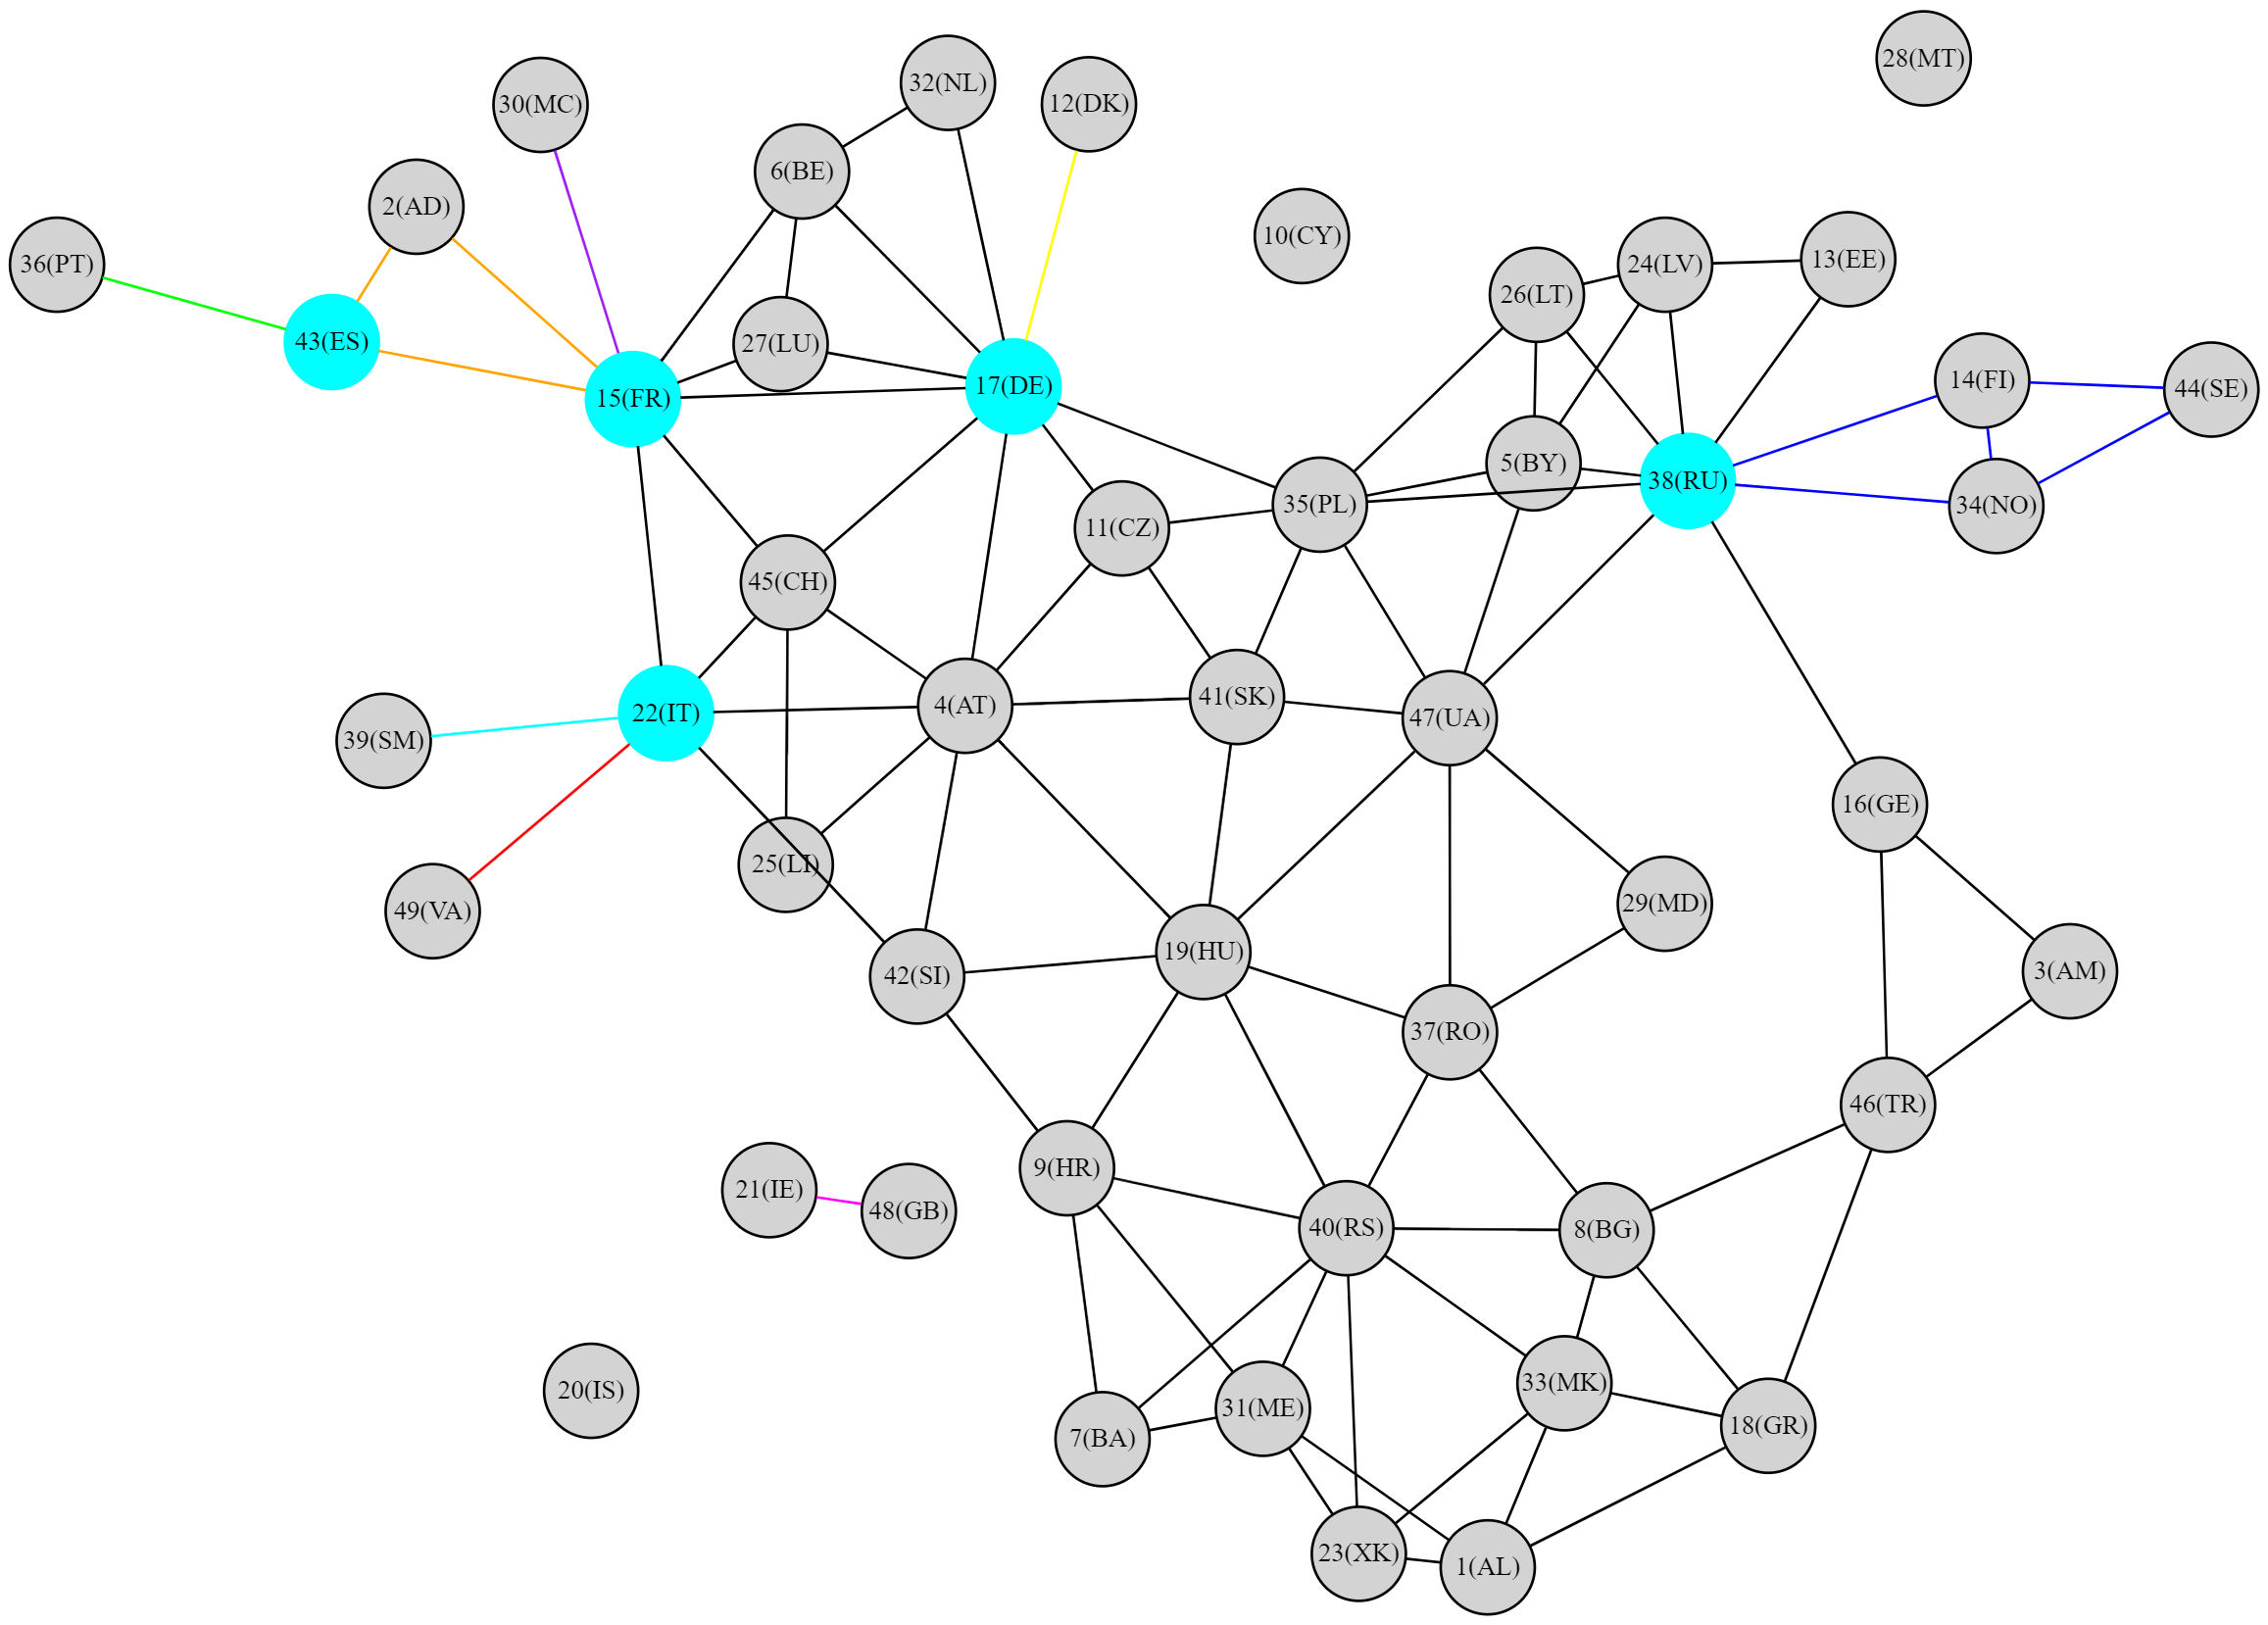
\includegraphics[width=1\textwidth]{blocks.png}
		\caption{Cut vertices are painted cyan, the edges of one block have the same color(black edges are also in the block)}
	\end{figure}
\begin{figure}[h]
	\centering
	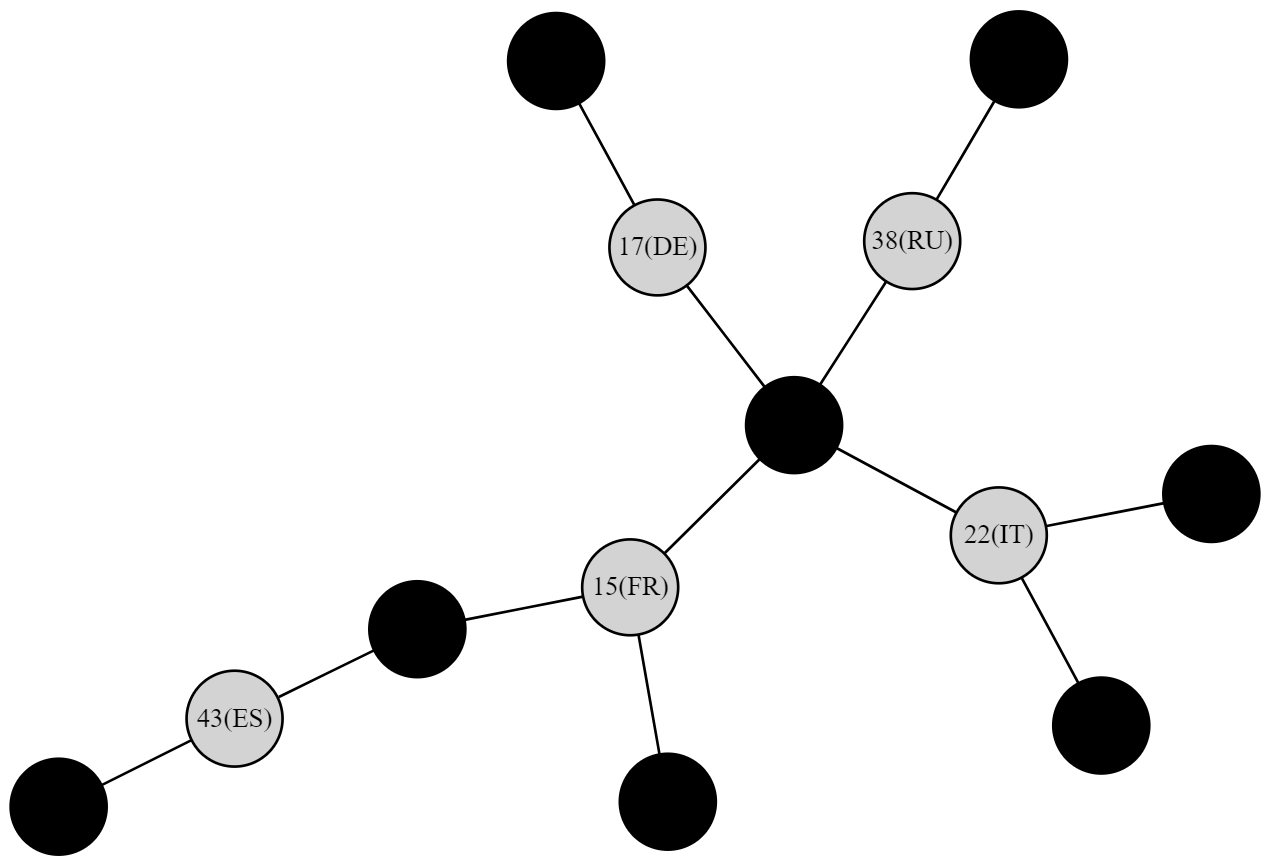
\includegraphics[width=1\textwidth]{block cut tree.png}
	\caption{Block-cut of $\mathcal{G}$ (black vertices are blocks, others are cut vertices)}
\end{figure}\newpage
	(m) fd
\end{document}
